
\newcommand{\LowLevelSystemSummary}{
    \begin{figure}[H] 
        \centering
        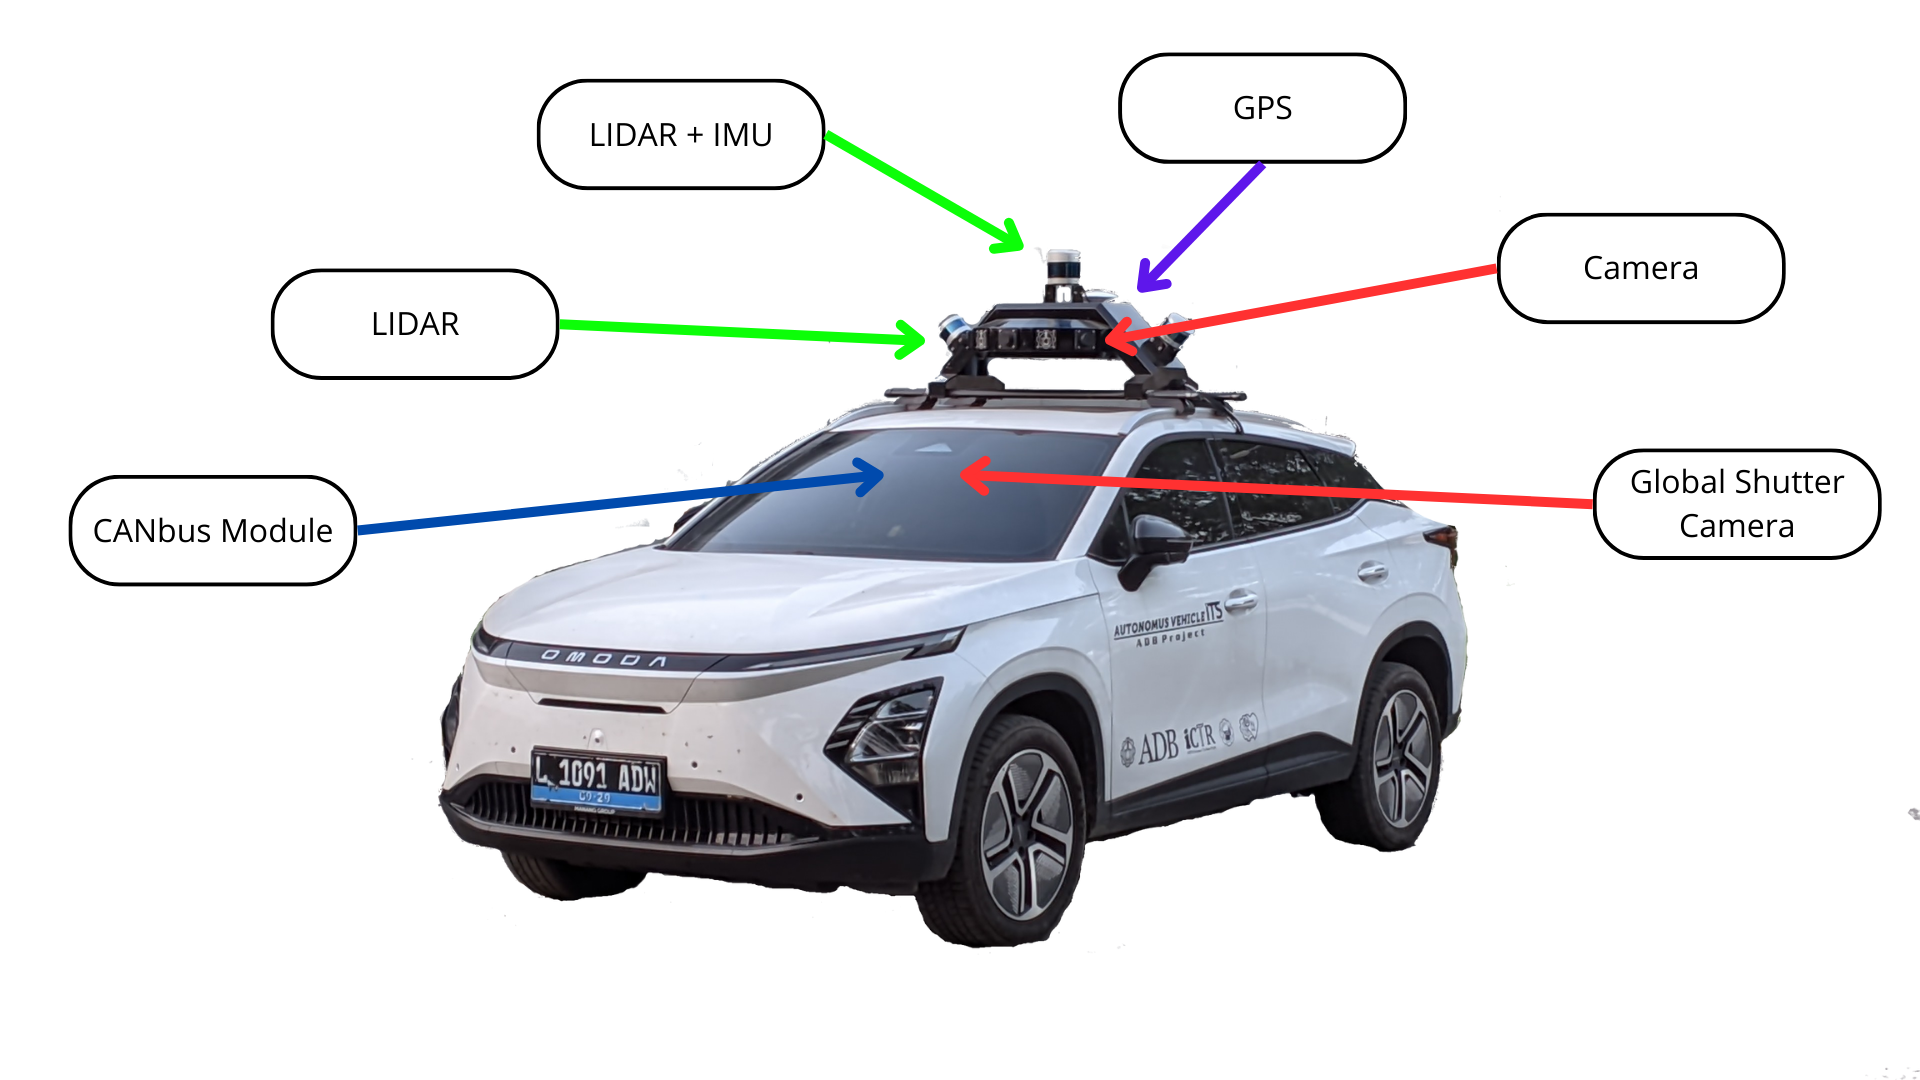
\includegraphics[width=\linewidth]{../konten/omoda_sys.png}
        \caption{Sensor Implementation on Icar}
        \label{fig:sensor_implementation}
    \end{figure}

    Icar with new system was implemented by modifying the fully conventional vehicle. The modification includes adding a new set of sensors and managing the main CANbus. Figure \ref{fig:sensor_implementation} shows the sensor implementation on Icar. The sensors used in this system include 2x LIDAR, 1x LIDAR with IMU, GPS, 3x RGB Camera, and 1x global shutter camera. 

    \begin{figure}[H] 
        \centering
        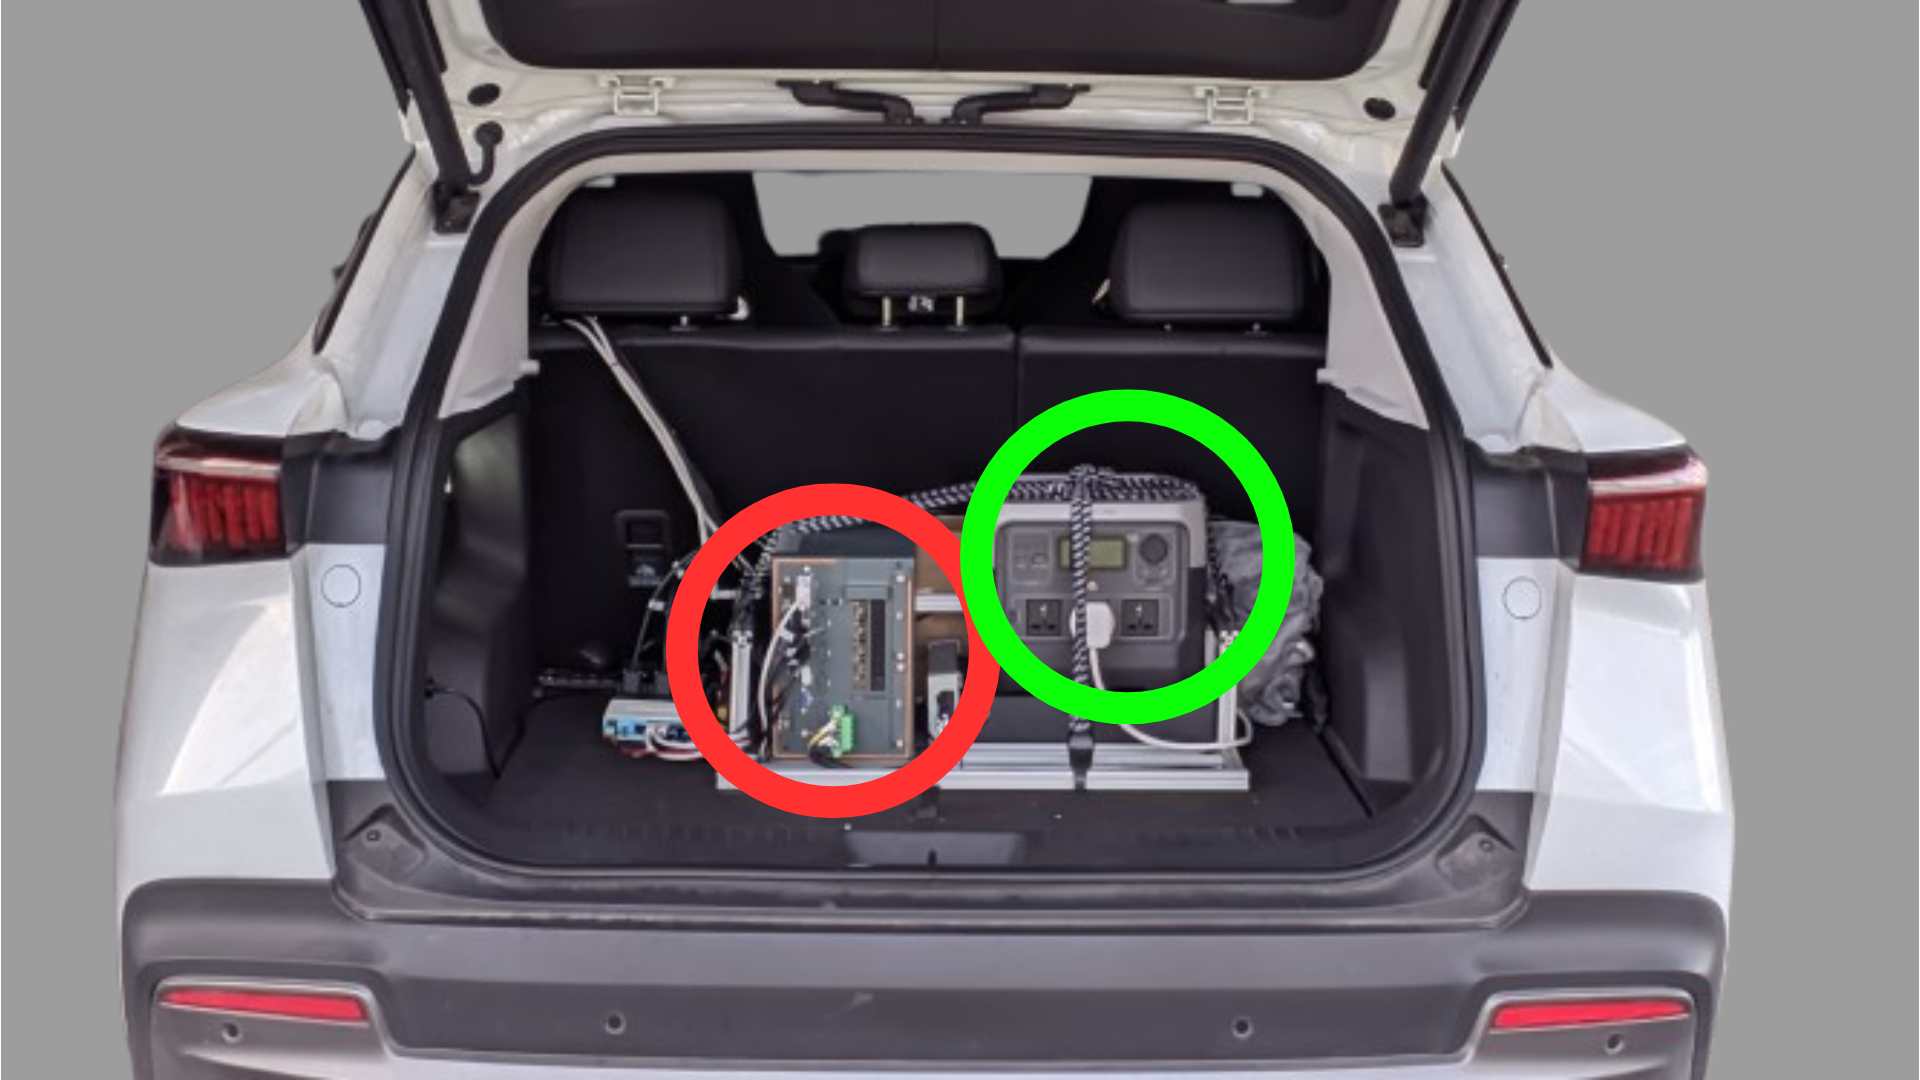
\includegraphics[width=\linewidth]{../konten/omoda_belakang.png}
        \caption{Computing Hardware}
        \label{fig:pc_omoda}
    \end{figure}

    Figure \ref{fig:pc_omoda} shows the hardware to do all the program and computation. The green circle is the power supply unit to supply power to the main computer and all the sensor based on \ref{fig:sensor_implementation}. The red circle is the main computer that installed inside the vehicle. 

}

\newcommand{\ImplementationofDepthImageCreation}{
    Based on figure \ref{fig:middleware_system}, the first major step is Depth Image Creation. This step convert all LIDAR point cloud data to the single depth image based on camera intrinsic. Figure \ref{fig:depth_image} shows the result of Depth Image Creation from LIDAR point cloud data.

    \begin{figure}[H] 
        \centering
        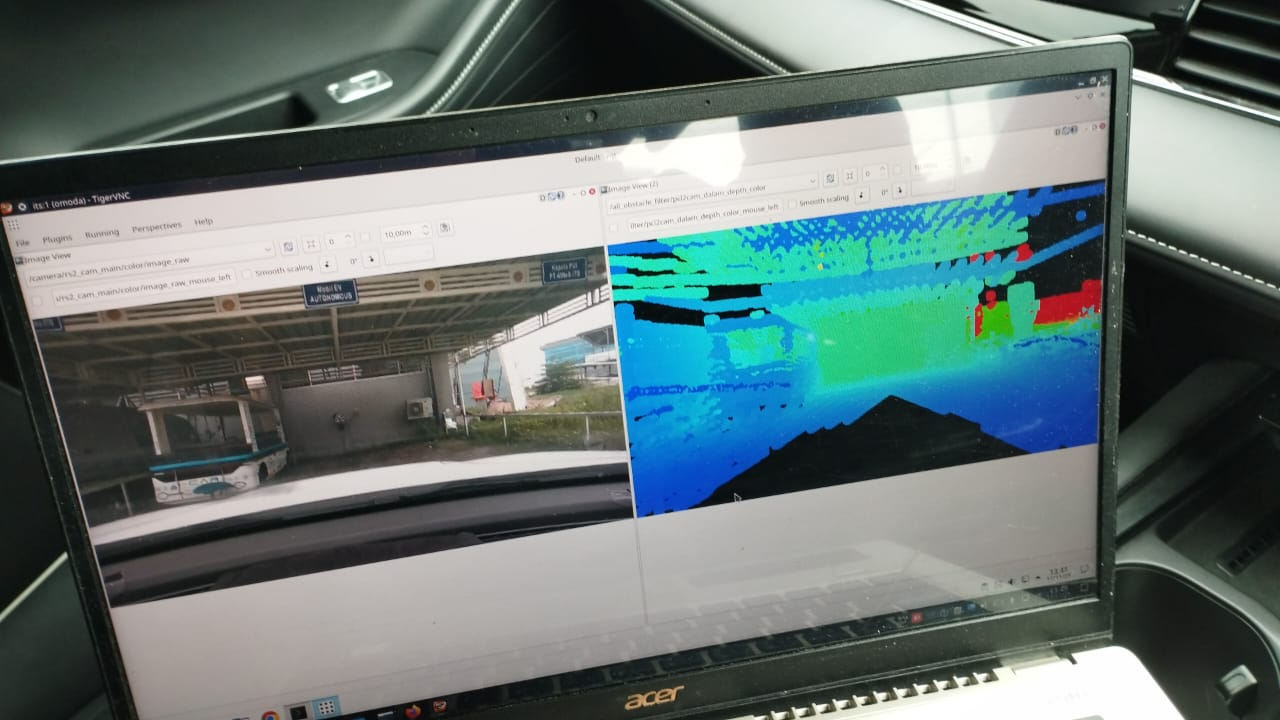
\includegraphics[width=\linewidth]{../konten/depth.jpeg}
        \caption{Result of Depth Image Creation}
        \label{fig:depth_image}
    \end{figure}

    In the figure \ref{fig:depth_image}, the left image is the RGB image from the camera, and the right image is the depth image created from LIDAR point cloud data. The depth image painted on Jet colormap, where the closer the distance to the camera, the color will be more blue, and the farther the distance to the camera, the color will be more red.
}

\newcommand{\ImplementationofRoadSegmentation}{
    \label{sec:implroadseg}
    Once we have trained our model using our training strategy on \ref{sec:model_training}, we can implement our model on to the vehicle. The first step is to load the model then inference the rgb image by that model. Figure \ref{fig:res_road_segmentation} shows the result of Road Segmentation from our model.

    \begin{figure}[H] 
        \centering
        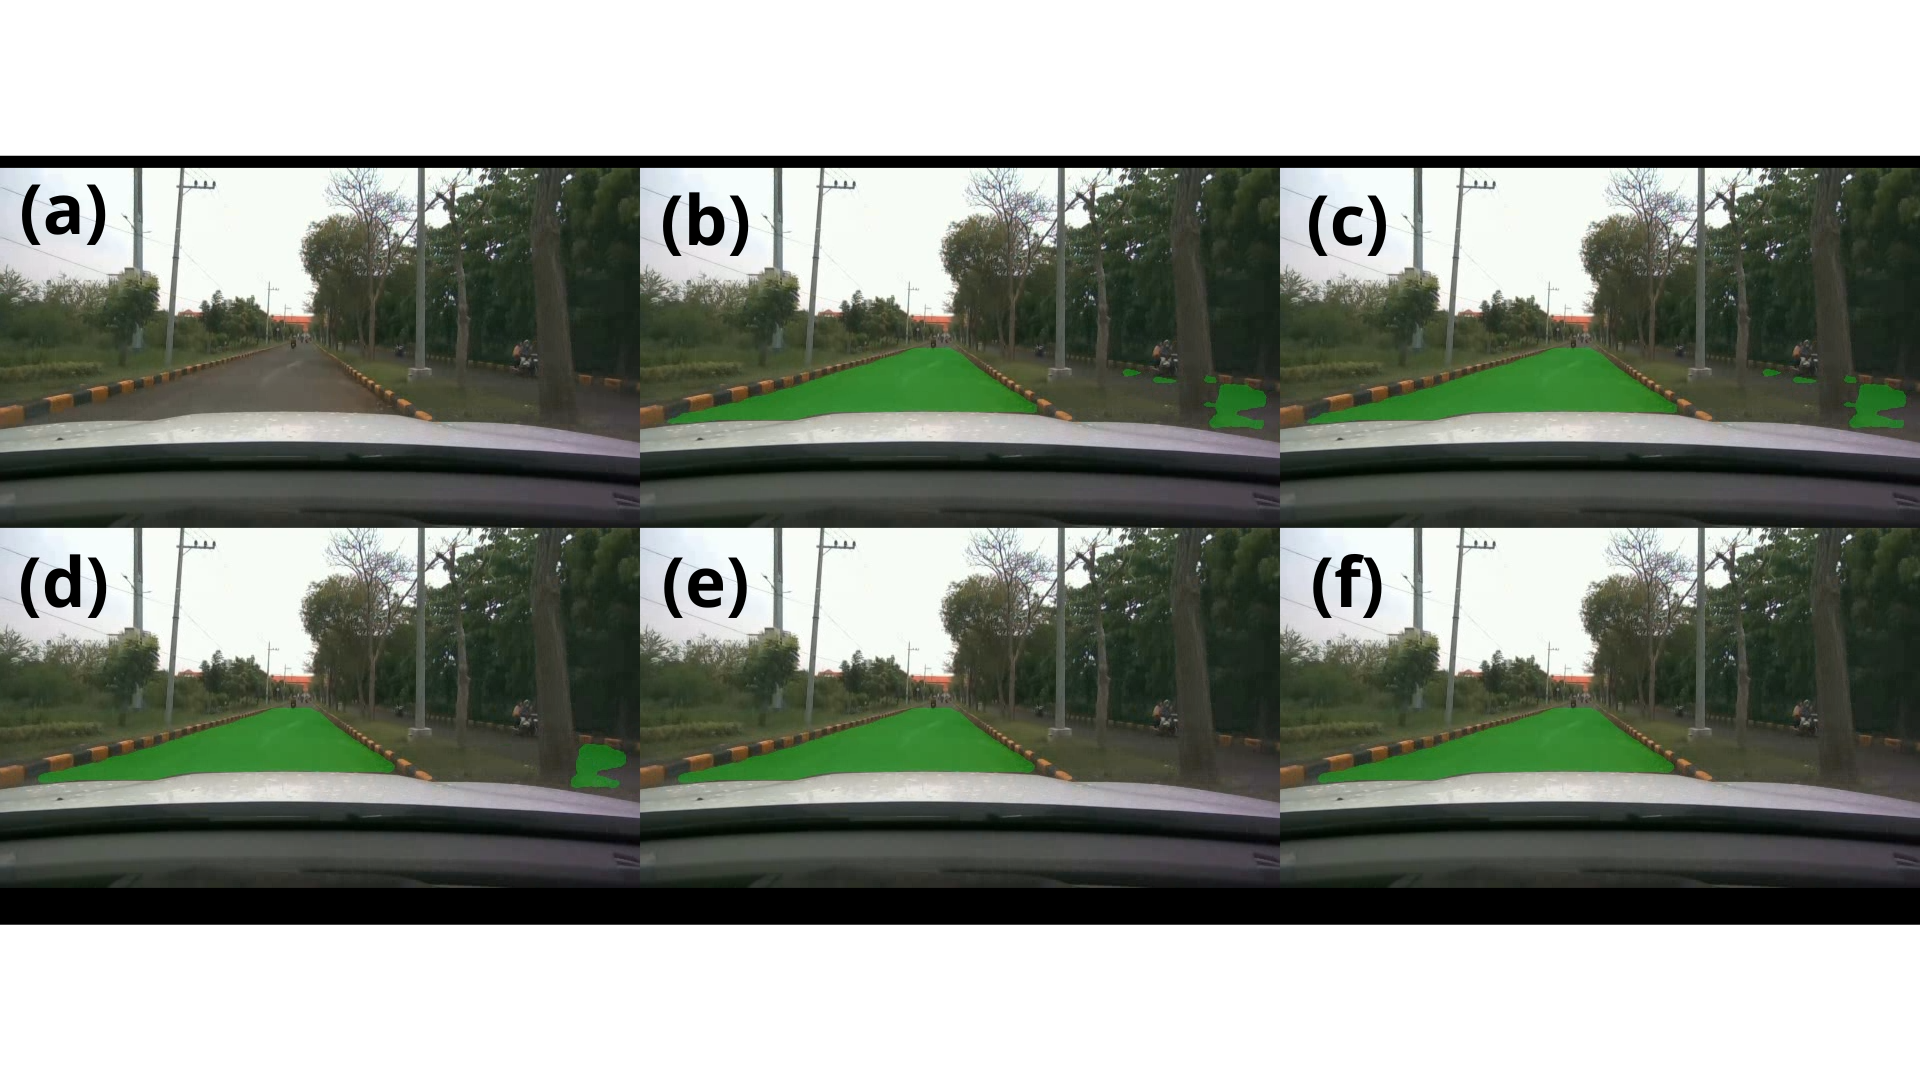
\includegraphics[width=\linewidth]{../konten/semua_canva.png}
        \caption{Result of Road Segmentation}
        \label{fig:res_road_segmentation}
    \end{figure} 

    In the figure \ref{fig:res_road_segmentation}, the sub image (a) is the RGB image from the camera, (b) is the raw Road Segmentation result from the model, (c) is the result of ROI cut process, (d) is the result of morphological operation process, (e) is the result of selecting the largest area, and (f) is the final Road Segmentation result after applying low pass temporal effect.  

    The last sub image (f) in figure \ref{fig:res_road_segmentation} is the final Road Segmentation result that will be used on the next step, which is transforming the Road Segmentation to the base link frame by using depth image from \ref{fig:depth_image}. Figure \ref{fig:res_road_segmentation_trans} shows the result of Road Segmentation transformation to the base link frame.

    \begin{figure}[H] 
        \centering
        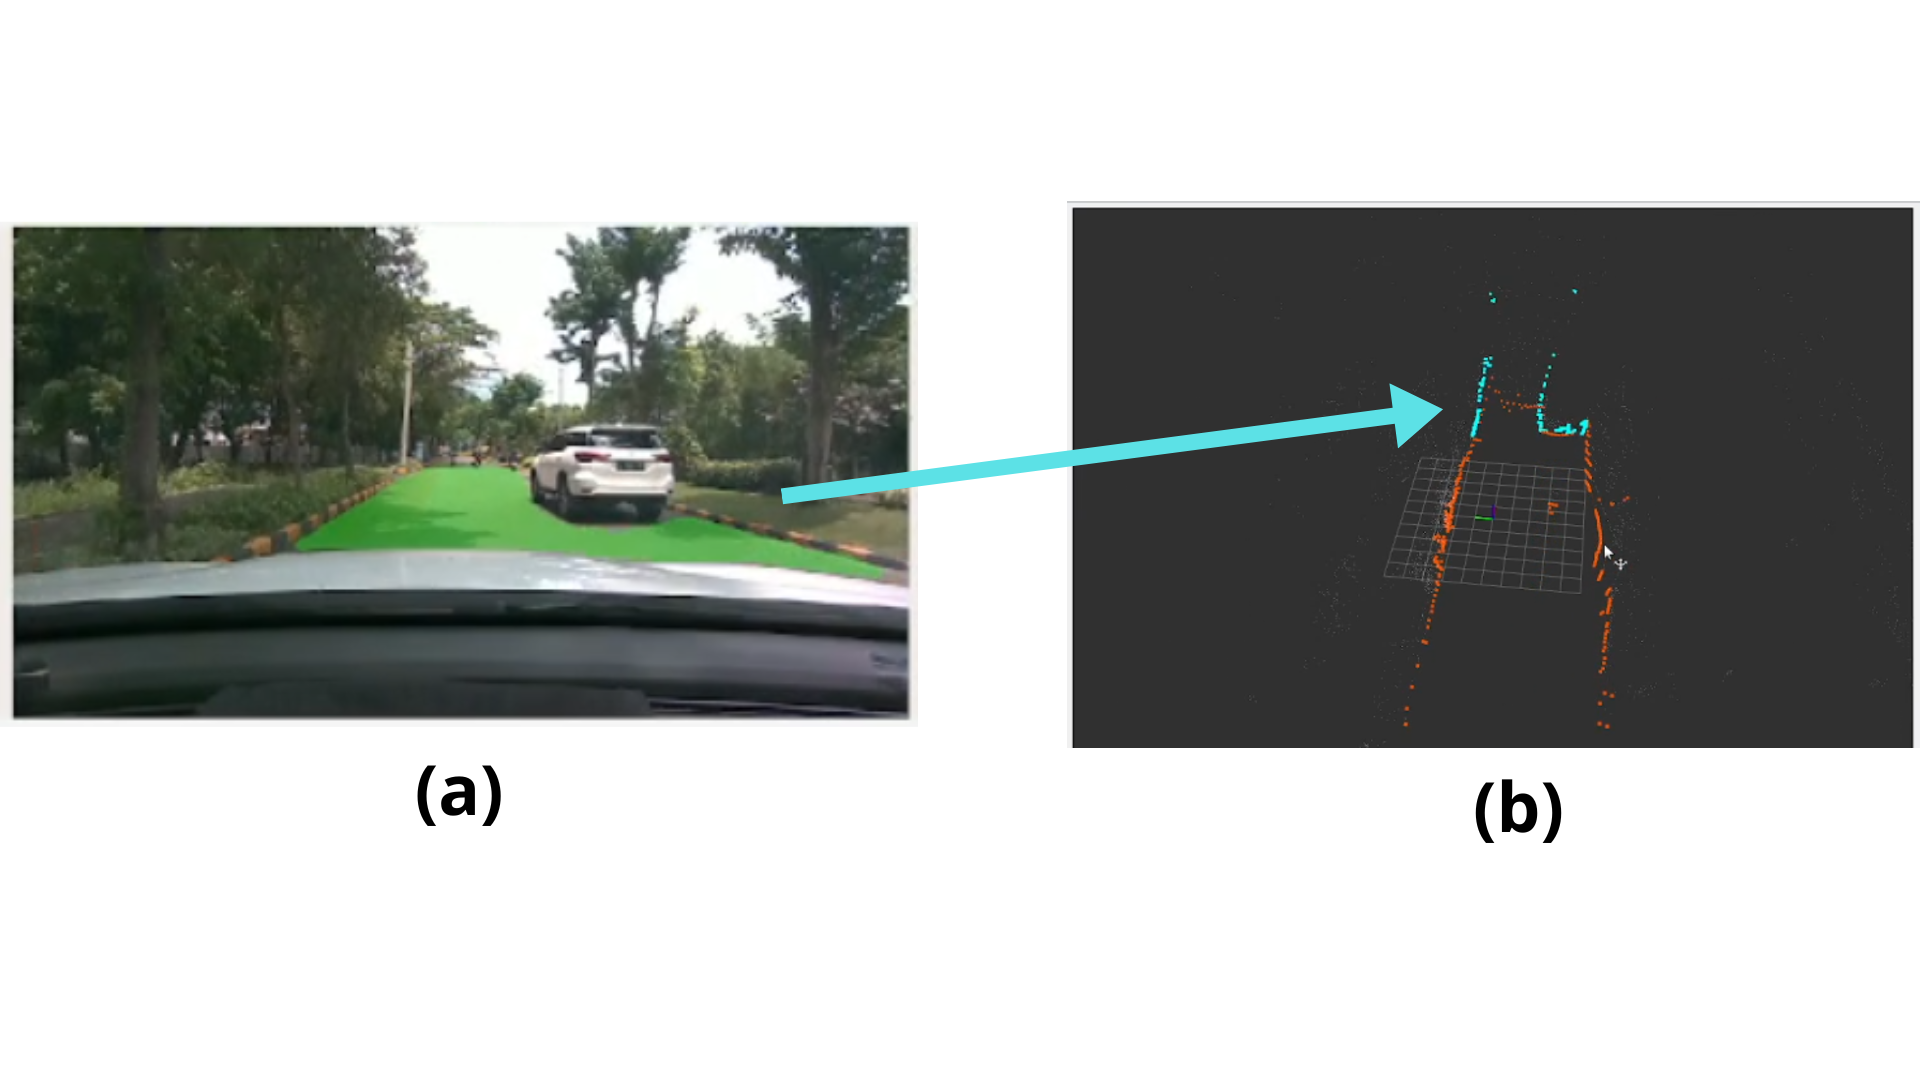
\includegraphics[width=\linewidth]{../konten/ssvid_terpilih.png}
        \caption{Result of Road Segmentation Transformation}
        \label{fig:res_road_segmentation_trans}
    \end{figure} 

    In the figure \ref{fig:res_road_segmentation_trans}, the sub image (a) is the segmented road image and (b) is the road point cloud laser scan in the base link frame. In sub image (b), the cyan point is the road point cloud that obtained from the transformation process. 
}

\newcommand{\ImplementationofGraphBasedSLAM}{
    \label{sec:implslam}
    Based on figure \ref{fig:middleware_system} and figure \ref{fig:graph_slam}, there are 5 inputs that going to Graph Based SLAM block: RGB Image, Depth Image from LIDAR, Road Laser Scan, GPS, and odometry. The GPS and odometry used to find and filter out nodes outside local-radius area for finding loop closures. Then, the RGB image and depth image from LIDAR used to find the loop closures by using Bag of Words method. The road laser scan used to calculate the constraint for GTSAM optimization process. The last step is doing pose fusion to produce high frequency pose estimation like we do before on \cite{ref_ku_icamimia}. 
    \par     
    The the first major step is synchronization. The synchronization has been done using approximate sync with delay tolerance 0.1 second. We have setup data queue size for synchronization up to 30, so it will be tolerance for various data update rate. 
    \par    
    The second step is the image feature extraction. The strategy that we used to do that is using ORB feature extraction. By combining it from the guess pose of GPS and odometry, we can create a Bag of Words that will be saved and proceed inside Nodes Processing. Figure \ref{fig:res_orb} shows the result of ORB feature extraction.

    \begin{figure}[H] 
        \centering
        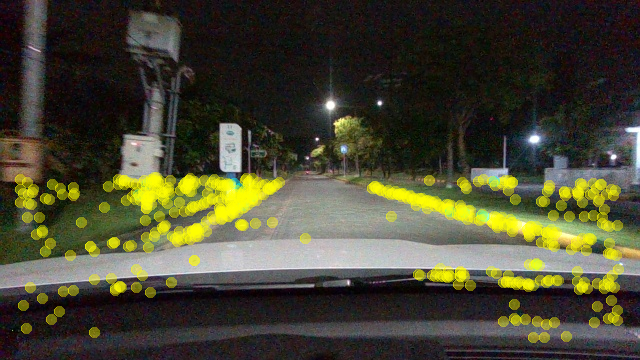
\includegraphics[width=\linewidth]{../konten/orb_1_saja.png}
        \caption{Result of ORB Feature Extraction}
        \label{fig:res_orb}
    \end{figure} 

    The figure \ref{fig:res_orb} shows the result of ORB feature extraction where the yellow points are the features that have been extracted using ORB algorithm. Those features will be converted into Bag of Words if the new node appear. 

    \par    
    The next step is to do registration from the current node into saved nodes. The image registration using ORB and RANSAC. The ORB will be found the same feature from current image in current node into the previous saved Bag of Words in saved nodes. Figure \ref{fig:res_orb_ransac} shows the result of image matching process.

    \begin{figure}[H] 
        \centering
        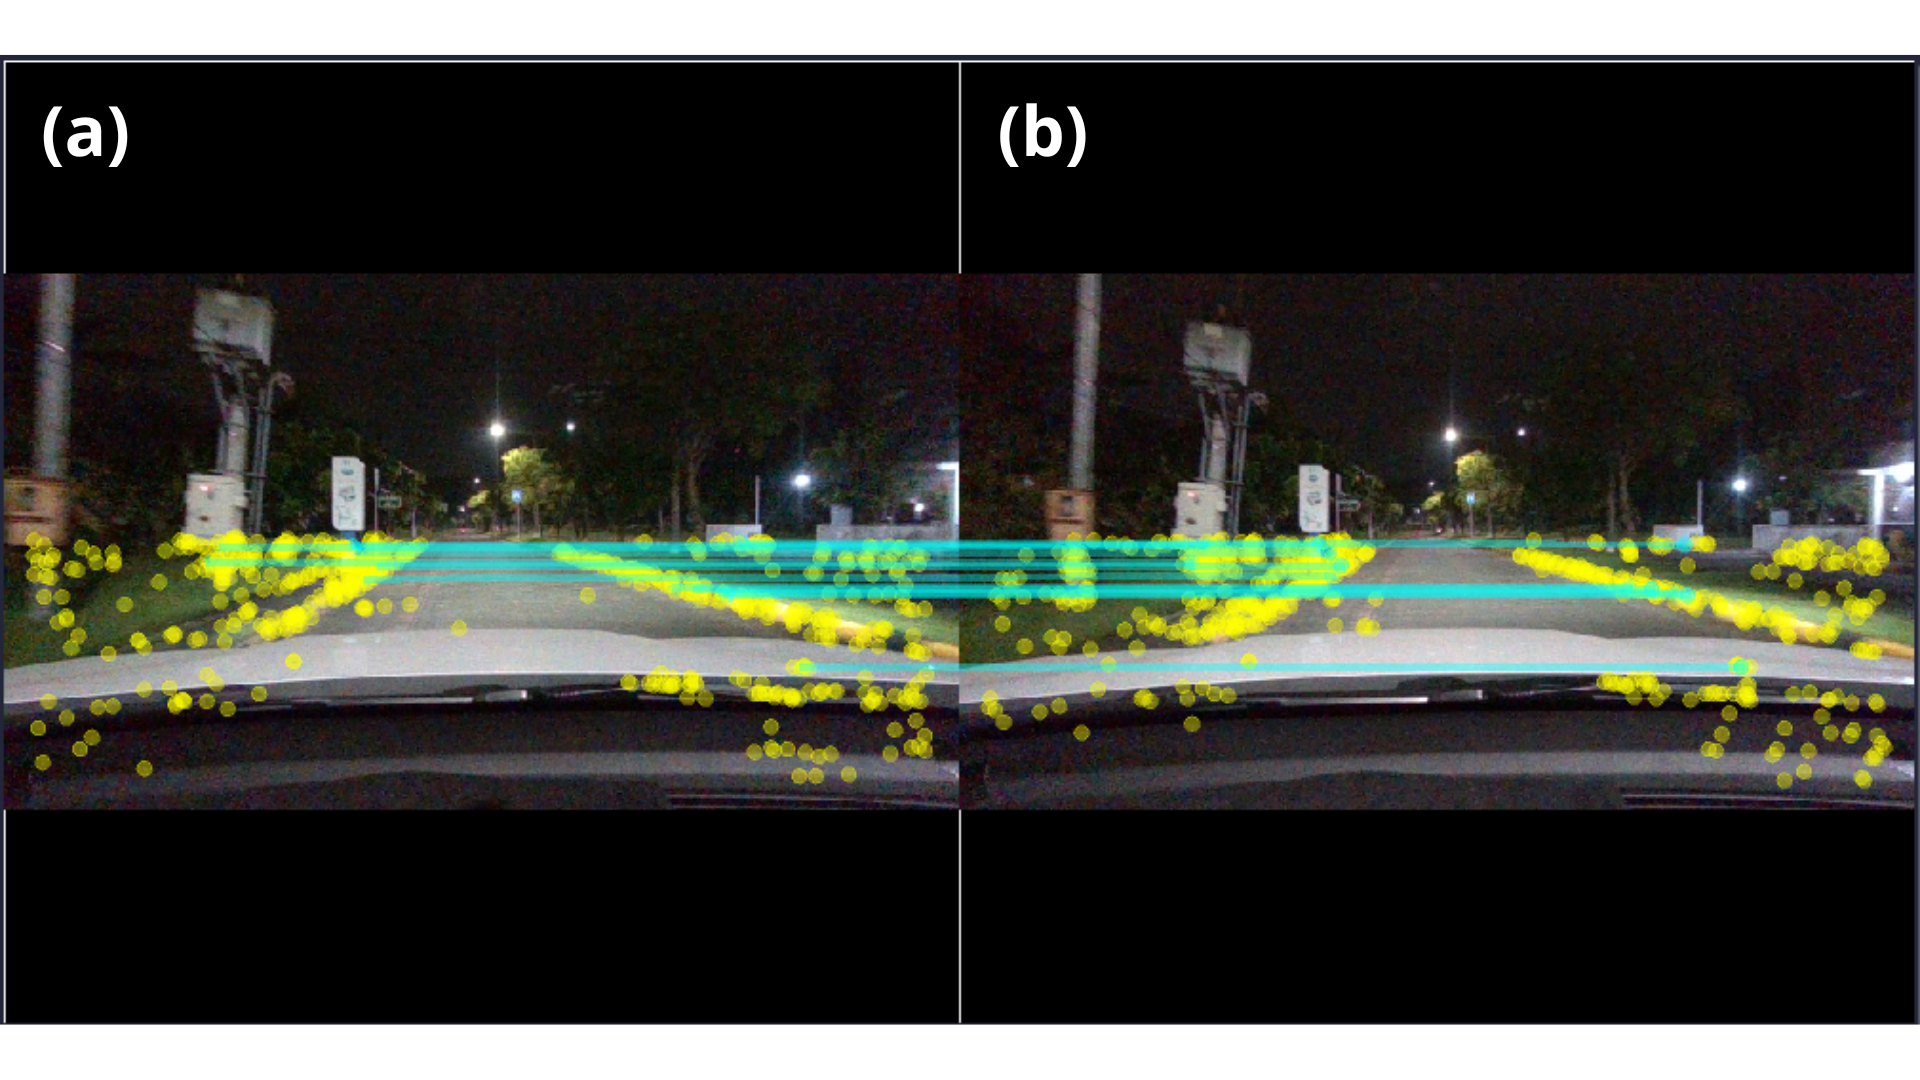
\includegraphics[width=\linewidth]{../konten/orb_malam_canva.png}
        \caption{Result of ORB and RANSAC}
        \label{fig:res_orb_ransac}
    \end{figure} 

    Figure \ref{fig:res_orb_ransac} shows the result of image matching process using ORB and RANSAC where the yellow points are the features for each images and the cyan line is the inliers detected and filtered using ORB and RANSAC. The sub image (b) is the current image in current node and the sub image (a) is the previous saved image in the database. 

    \par   
    After we have found the inliers, the next step is thresholding the number of inliers found. If the number of inliers found more than the threshold, the loop closure hypothesis will be added. In the other hand, the strategy for the registration constraint in GTSAM optimization process is using ICP (Iterative Closest Point) algorithm between the current road laser scan and the previous saved road laser scan in the database. 

    \par    
    The final output of GTSAM Optimization process is the optimized pose estimation. That optimized pose estimation will be fused with high frequency odometry to produce high frequency pose estimation using Kalman Filter. The strategy that we used is by setting the odometry as a prediction by doing a difference between the current odometry and the previous odometry. Then, the optimized pose estimation from GTSAM will be used as a correction measurement for Kalman Filter.
}

\newcommand{\ImplementationofNavigationSystem}{
    The implementation of navigation system is divided into three parts. The first part is global navigation estimation. The second part is local navigation estimation. The last part is the safety system implementation. 

    \par     

    The global navigation estimation is implemented by using the pose estimated from the implementation of graph based SLAM \ref{sec:implslam} and the 3rd party system that produces waypoints to target navigation. By doing a window filter for 20 m, we can filter the waypoint within 20 m radius from the estimated pose. After we have a filtered waypoints, the next step is to convert that waypoint into meter level coordinate based on base link using haversine formula. The result from that process will produce a trajectory called global trajectory. Figure \ref{fig:nav_global} shows the result of global navigation estimation.

    \begin{figure}[H] 
        \centering
        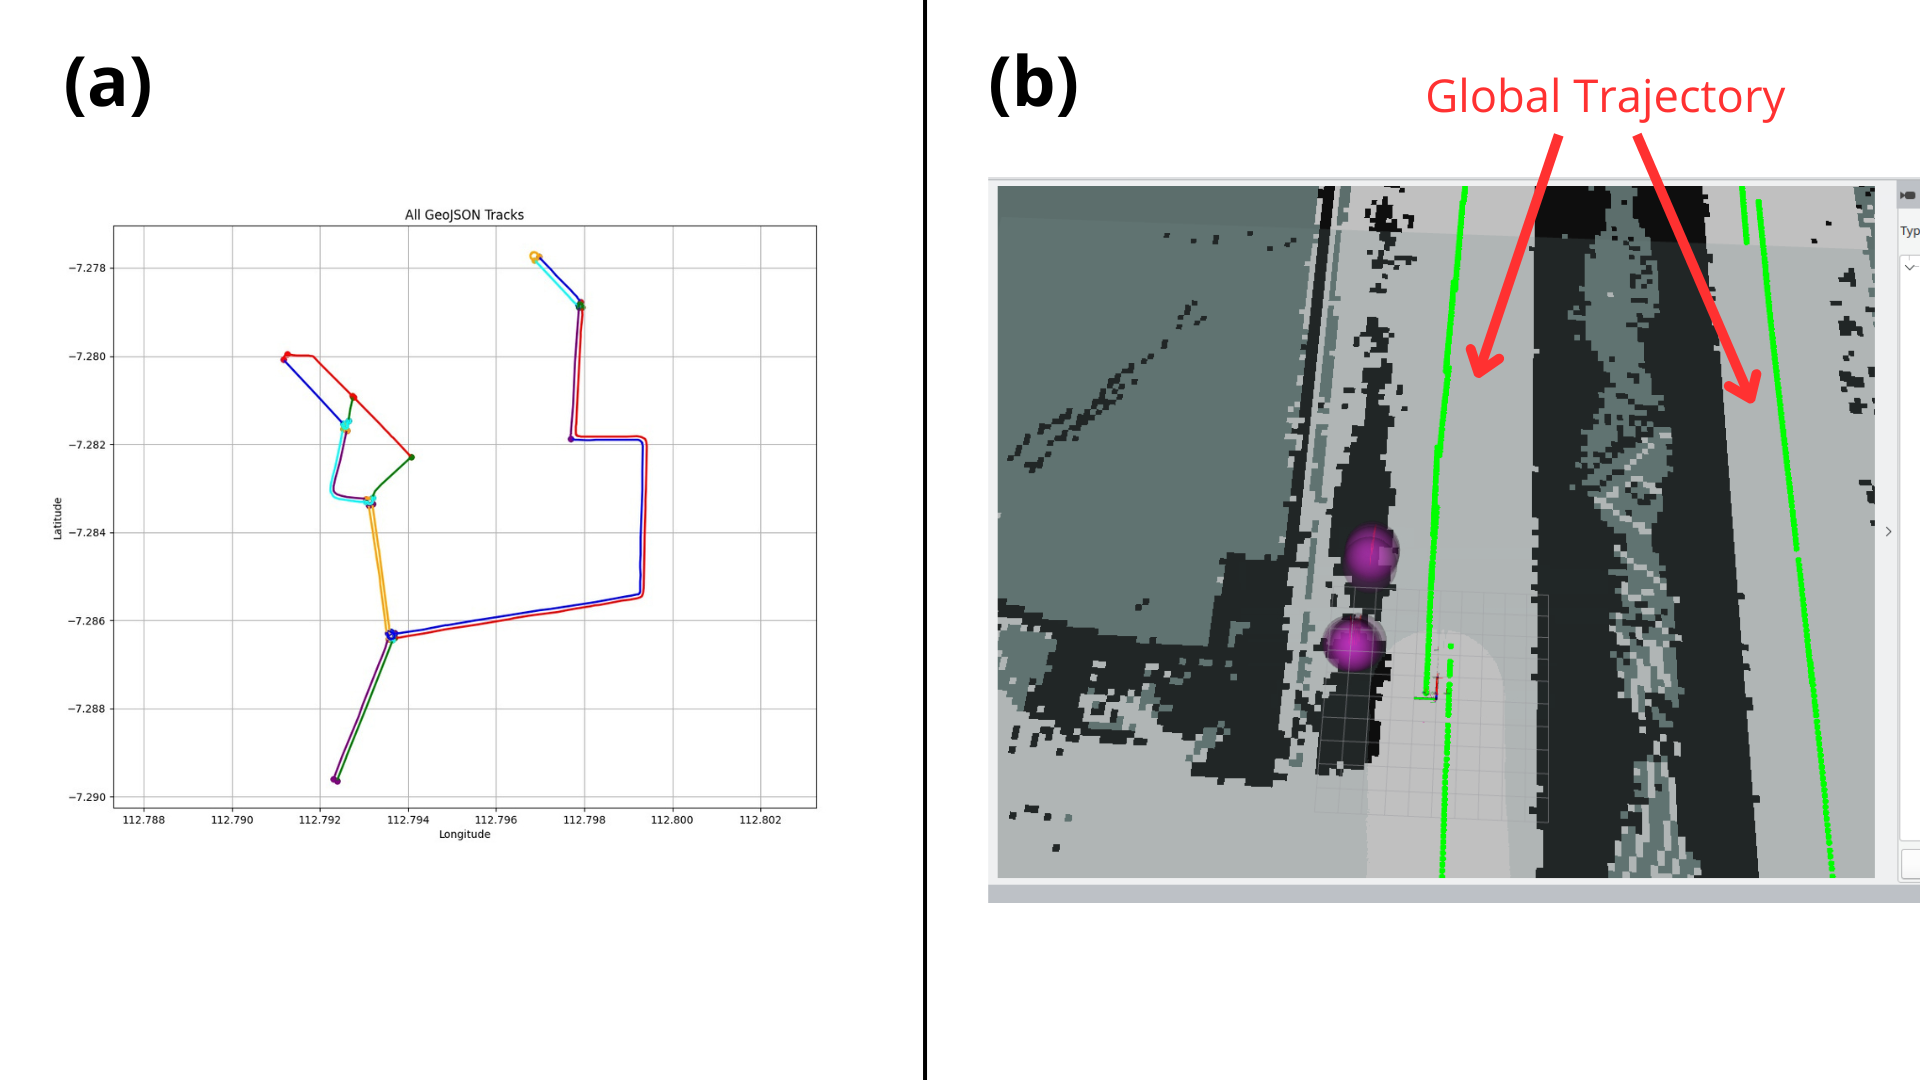
\includegraphics[width=\linewidth]{../konten/gps_hernanda3.png}
        \caption{Result of Global Navigation Estimation}
        \label{fig:nav_global}
    \end{figure} 

    The sub image (a) in the figure \ref{fig:nav_global} is the full path target that coming from 3rd party system. The sub image (b) is the global trajectory that will be used to compute next action. The global trajectory represented by the green line points inside sub image (b).

    \par    

    The next step is local navigation system that will produces a local trajectory and target velocity and steering. 
    Figure \ref{fig:nav_local} shows the result of the local navigation estimation.

    \begin{figure}[H] 
        \centering
        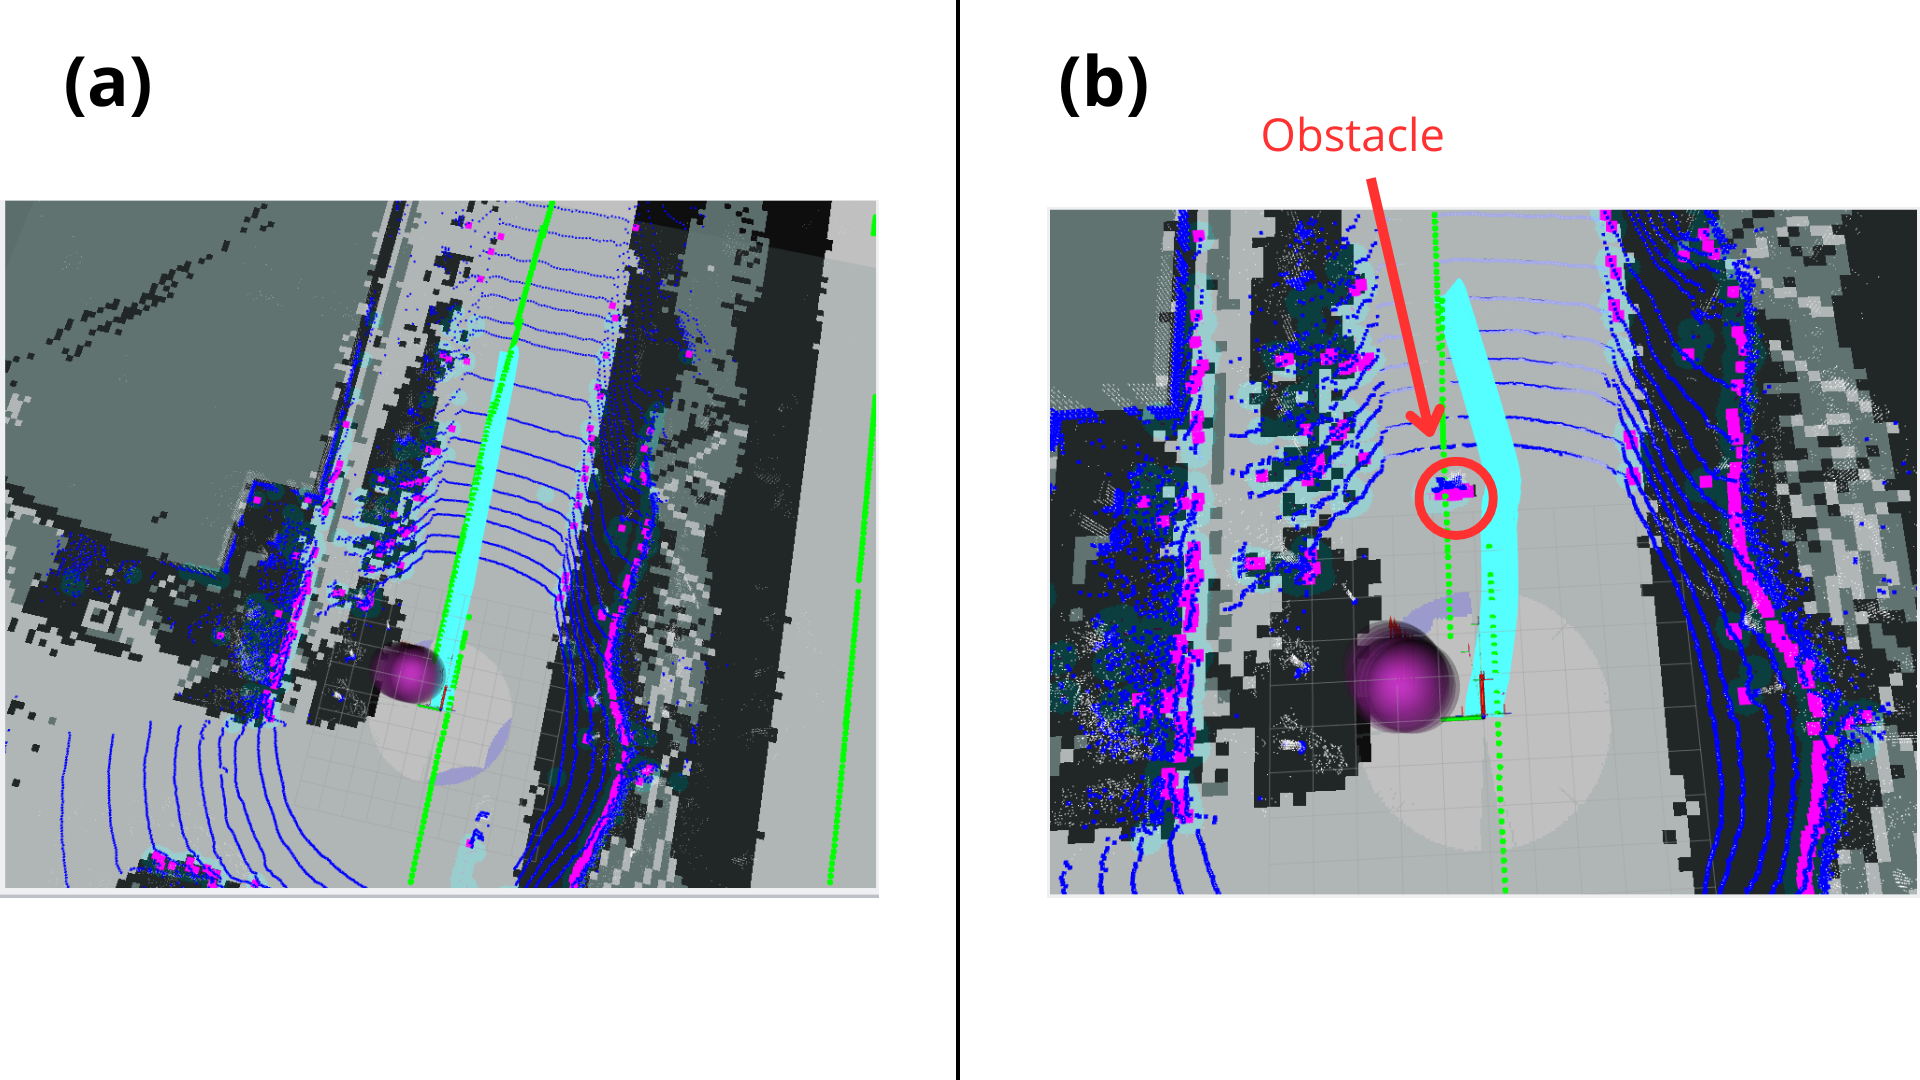
\includegraphics[width=\linewidth]{../konten/gps_loc2.png}
        \caption{Result of Local Navigation Estimation}
        \label{fig:nav_local}
    \end{figure} 

    In the figure \ref{fig:nav_local}, both sub image (a) and (b) represent the result of local navigation estimation. The sub image (a) is the local navigation system that follow the generated global trajectory without any obstacles. The sub image (b) is the local navigation system that obstructed by an obstacle. From the figure \ref{fig:nav_local}, we can see that the local trajectory (the cyan line points) in sub image (b) is avoiding the obstacle (the red area) by planning a new local trajectory that avoid the obstacle. 
    % \par     

    % The last step is implementing the safety system. 
}

\newcommand{\ResultofRoadSegmentation}{
asd
}


\newcommand{\SegmentationAccuracy}{
    The segmentation accuracy is measured by using Intersection over Union (IoU) metric. The IoU metric is calculated by dividing the intersection area between the predicted segmentation and the ground truth segmentation with the union area between the predicted segmentation and the ground truth segmentation. Table \ref{tab:iou_acc} shows the IoU segmentation accuracy result at different epoch during the training process.

    \begin{table}[H]
        \centering
        \caption{IoU Segmentation Accuracy Result}
        \label{tab:iou_acc}
        \begin{tabular}{|c|c|}
            \hline
            \textbf{Epoch} & \textbf{IoU} \\ \hline
            150 & 0.7697 \\ \hline
            200 & 0.7760 \\ \hline
            300 & 0.7831 \\ \hline
            \textbf{400} & \textbf{0.7928} \\ \hline
            500 & 0.7867 \\ \hline
        \end{tabular}
    \end{table}

    Table \ref{tab:iou_acc} shows that the best IoU segmentation accuracy is achieved at epoch 400 with IoU value of 0.7928. This model will be used for the implementation on the vehicle. 
    \par    

    It is considered that the IoU calculation for accuracy measurement is adequate enough because in real world application, there is a dimention called time. The IoU calculation for table \ref{tab:iou_acc} is calculated by selecting several random images that not included in the training dataset. But in real world application, the model will receive a continuous stream of images from the camera. So, we cannot trust only on the IoU calculation for several random images. We need to consider the temporal effect in real world application. The next section will discuss about the Importance of temporal effect in Road Segmentation application.
}

\newcommand{\TheImportantofTemporalEffect}{
    Like we discuss before, in real world application, the model will receive a continuous stream of images from the camera. So, we need to consider the temporal effect in real world application. The temporal effect that we imply in our model is using GRU (Gated Recurrent Unit) that will always save the global h state from the previous frame to the next frame. Figure \ref{fig:temporal_effect_gru} shows the comparison between with GRU temporal effect and without temporal effect in our Road Segmentation model.

    \begin{figure}[H] 
        \centering
        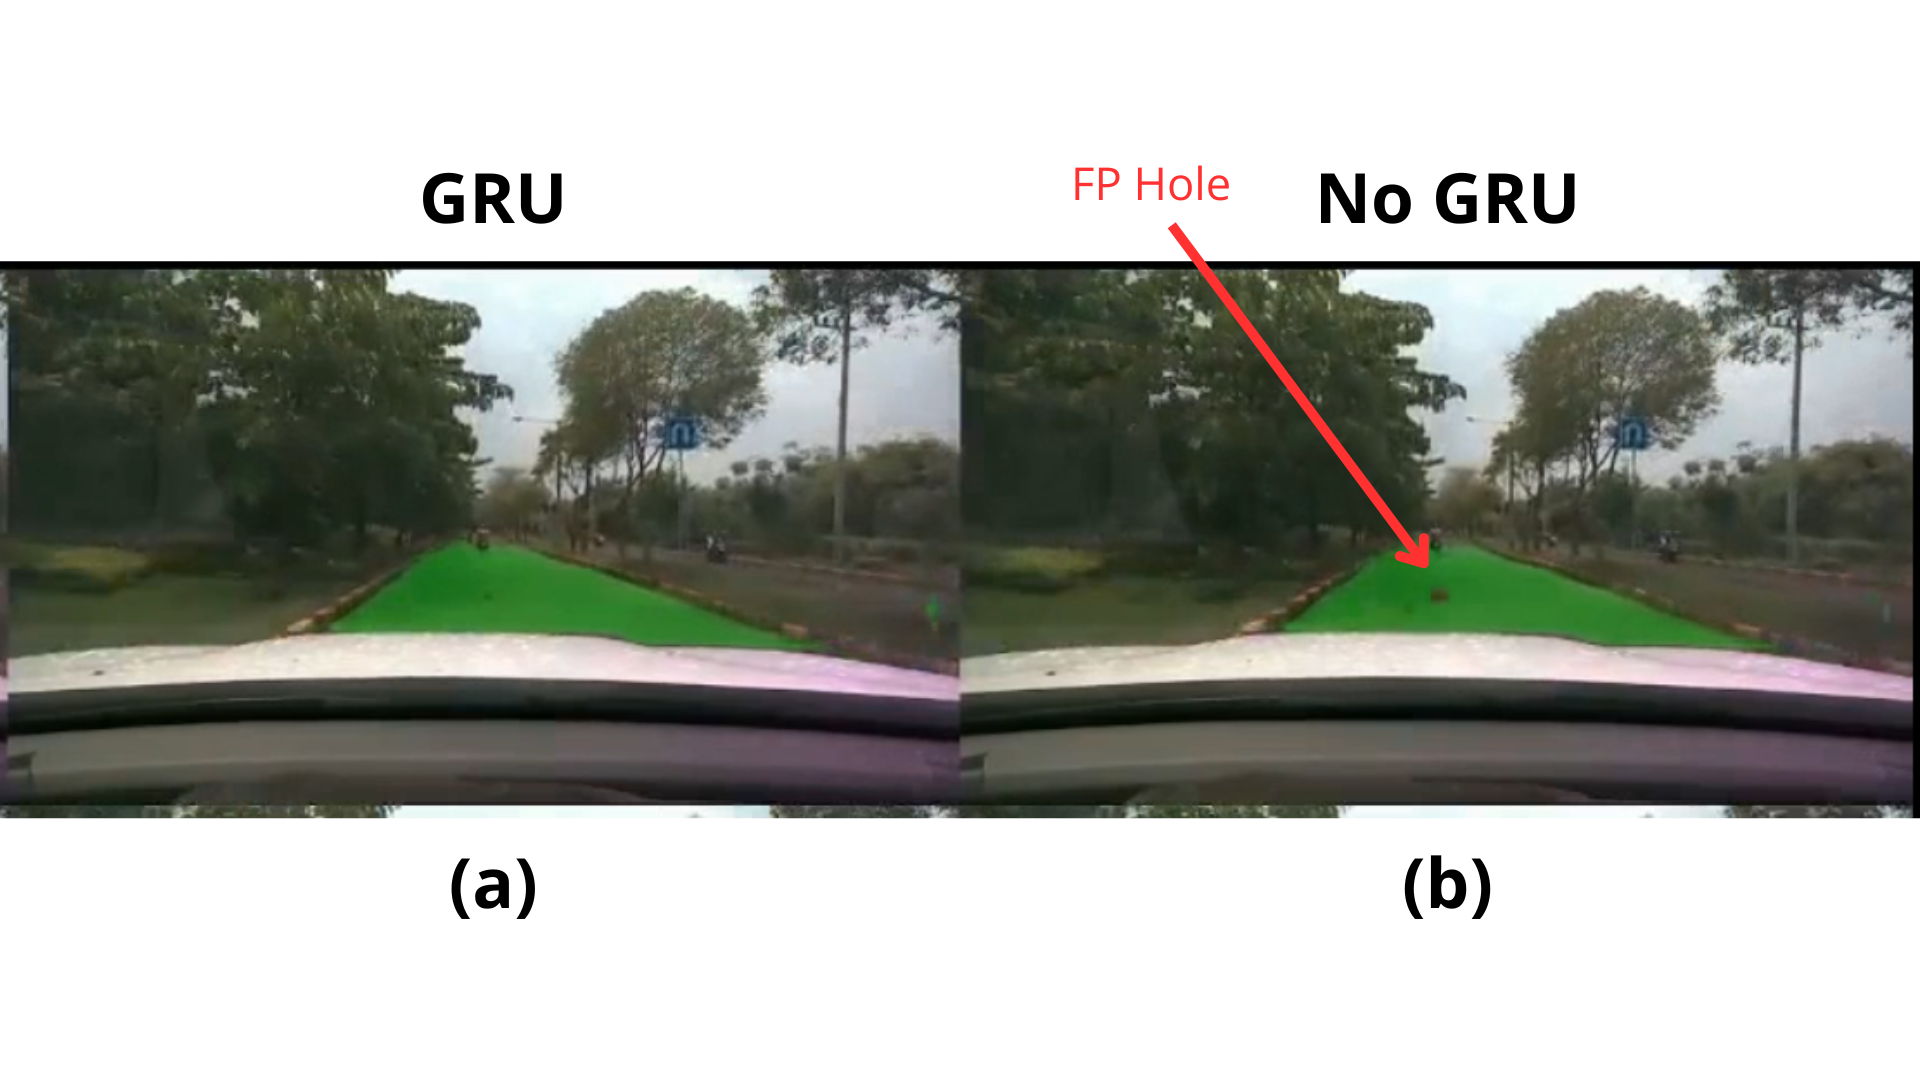
\includegraphics[width=\linewidth]{../konten/arghh_canva.png}
        \caption{With GRU Temporal Effect vs Without Temporal Effect}
        \label{fig:temporal_effect_gru}
    \end{figure} 

    In the figure \ref{fig:temporal_effect_gru}, the sub image (a) is the result of raw Road Segmentation using GRU and sub image (b) is the result of raw Road Segmentation without using GRU. All that mask captured without being post processed so we can analyze the effect of GRU temporal effect only. From the figure \ref{fig:temporal_effect_gru}, we can see that there is a hole called False Positive in sub image (b) because it does not use GRU temporal effect. That False Positive hole can be dangerous in real world application because it can mislead the navigation system to think that the area is not drivable area. 

    \par    
    Sometimes, even though we have used GRU temporal effect, there is a chance that the False Positive hole still appears in the Road Segmentation. Figure \ref{fig:temporal_effect_gru2} shows another example of False Positive hole that appear even though we have used GRU temporal effect.

    \begin{figure}[H] 
        \centering
        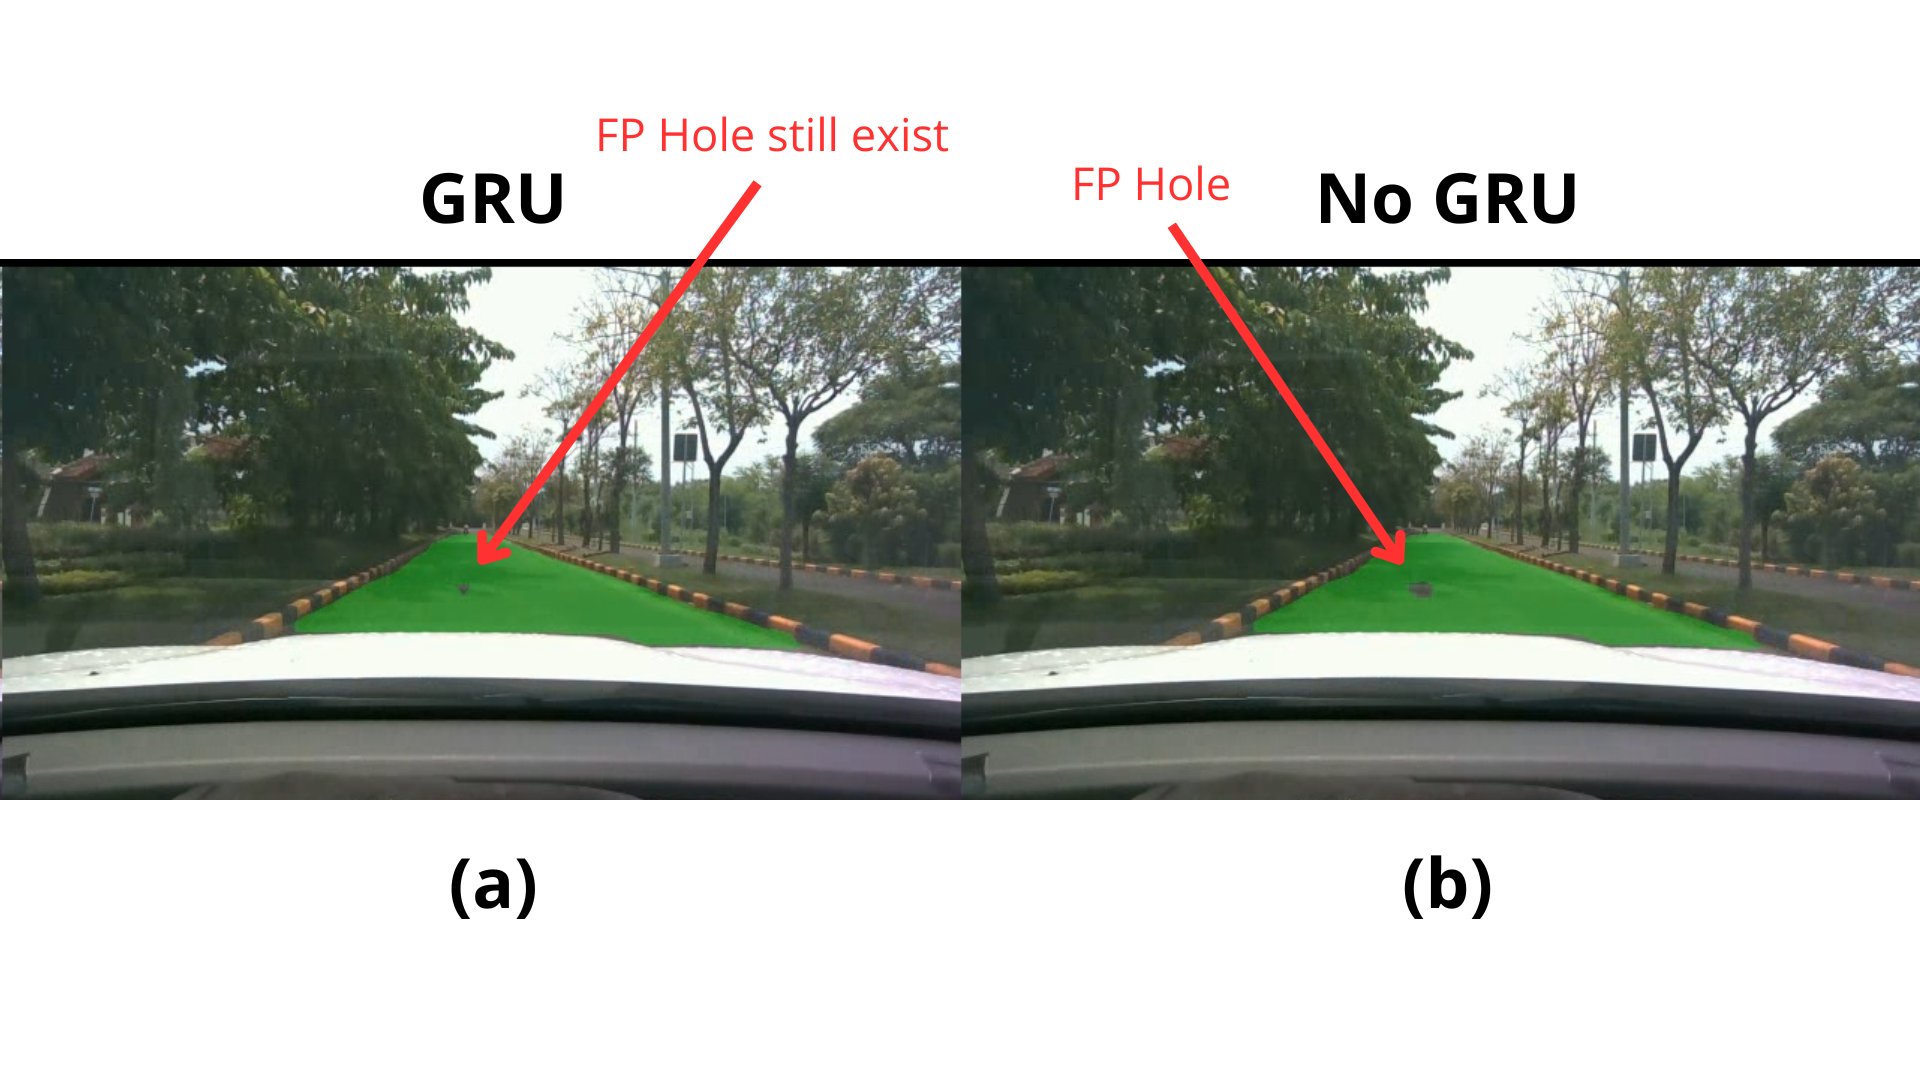
\includegraphics[width=\linewidth]{../konten/arghh_canva2.png}
        \caption{Another With GRU Temporal Effect vs Without Temporal Effect}
        \label{fig:temporal_effect_gru2}
    \end{figure} 

    Same as figure \ref{fig:temporal_effect_gru}, in the figure \ref{fig:temporal_effect_gru2}, the sub image (a) is the result of raw Road Segmentation using GRU and sub image (b) is the result of raw Road Segmentation without using GRU. All that mask captured without being post processed so we can analyze the effect of GRU temporal effect only. From the figure \ref{fig:temporal_effect_gru2}, we can see that there is a hole called False Positive in sub image (a) even though it smaller than the False Positive hole in sub image (b). To handle this case, we need to apply the post processing step to filter out the False Positive hole in the Road Segmentation result. The next section will discuss about the important of post processing in our Road Segmentation application.
}

\newcommand{\TheImportantofPostProcessing}{
    Like we discuss before, we have a problem called False Positive hole that appear in the Road Segmentation result even though we have used GRU temporal effect. We think it was a flickering problem that sometime happen in real world application. To handle this problem, we found out to apply a low pass filter over time. The idea is calculate per pixel value in frame t by the effect of previous frame t-1. The equation is shown below:

    \begin{equation}
        S_t(x,y) = \alpha \cdot S_{t-1}(x,y) + (1 - \alpha) \cdot S_{t}(x,y)
        \label{eq:lpf_temporal}
    \end{equation}

    where S is the segmentation mask, t is the current frame, t-1 is the previous frame, (x,y) is the pixel coordinate, and $\alpha$ is the low pass filter coefficient that we set to 0,1. After calculate pixel value, we divide it to binary value by thresholding it with 0.5 value. Figure \ref{fig:lpf_effect} shows the effect of post processing using low pass temporal filter.

    \begin{figure}[H] 
        \centering
        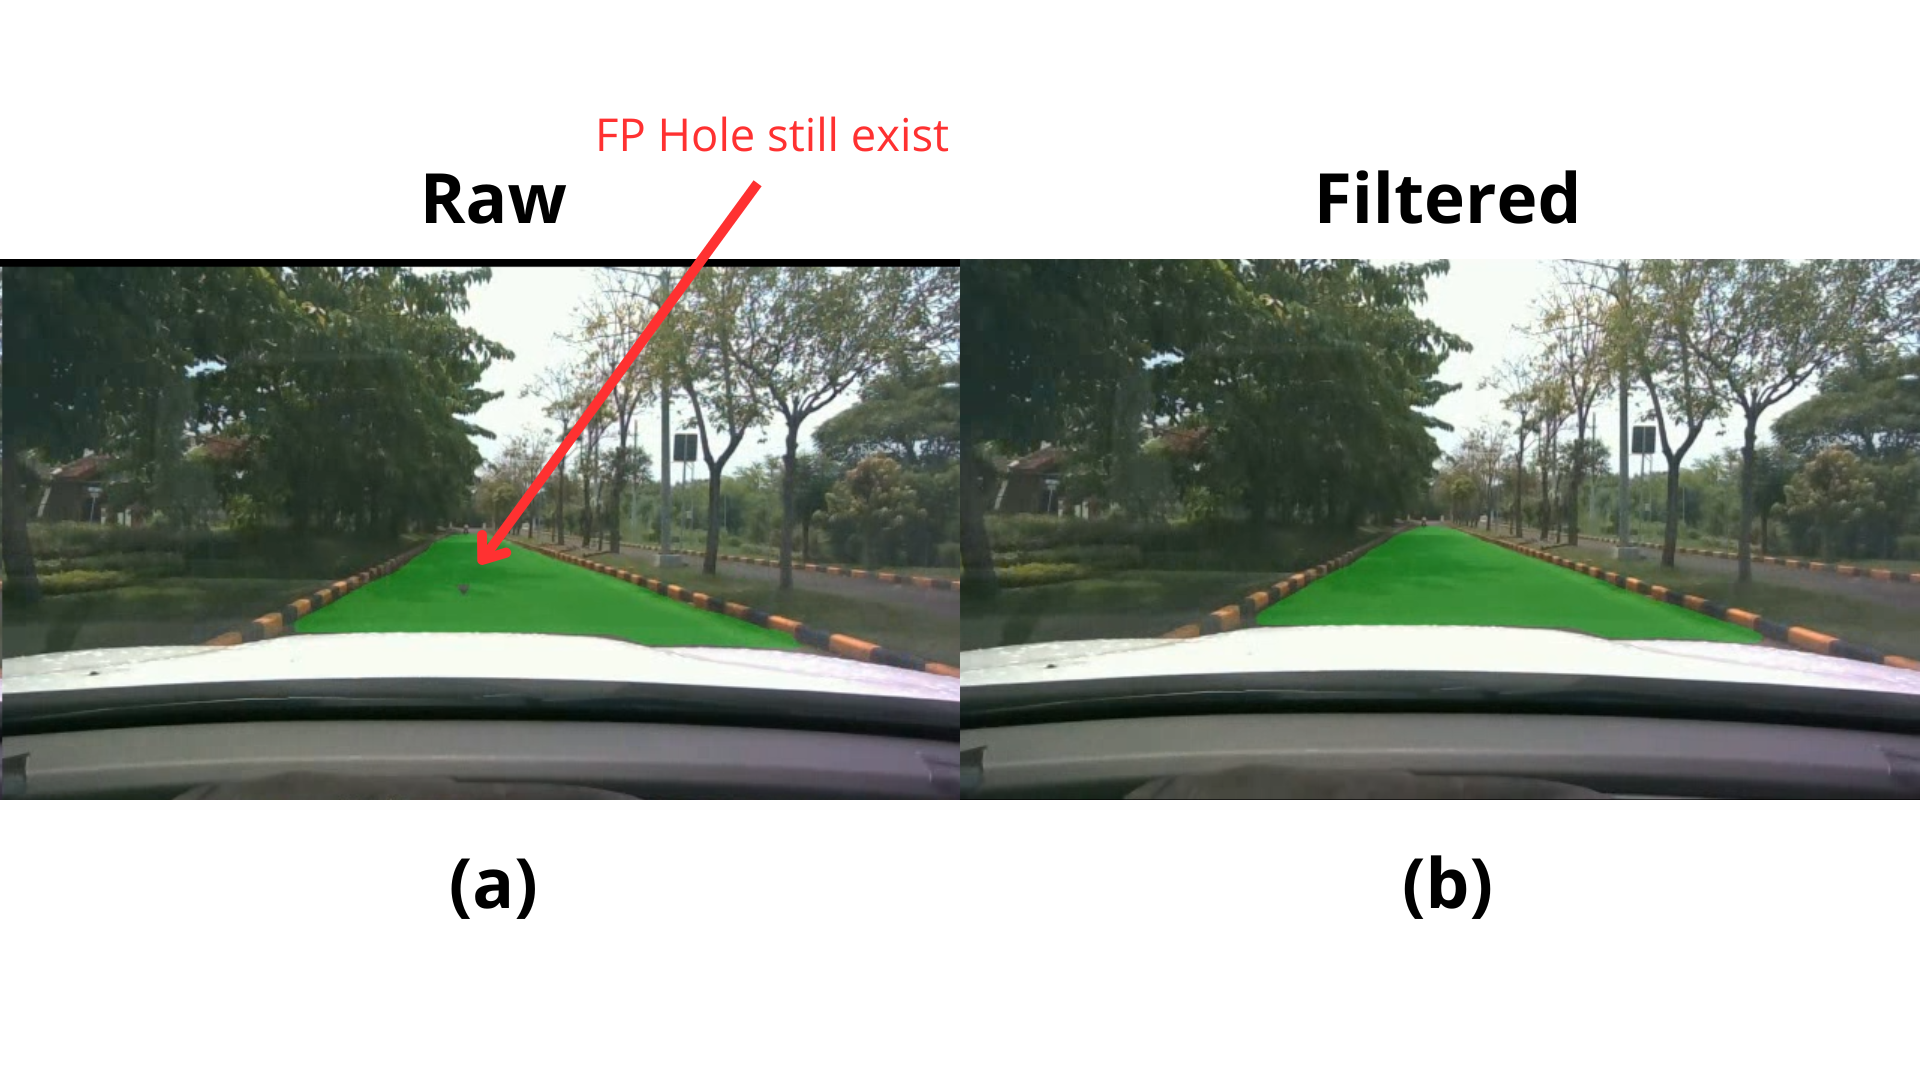
\includegraphics[width=\linewidth]{../konten/lpfff.png}
        \caption{Raw vs Low Pass Temporal Filtered Road Segmentation}
        \label{fig:lpf_effect}
    \end{figure} 

    In the figure \ref{fig:lpf_effect}, the sub image (a) is the raw Road Segmentation result from the model, and (b) is the Road Segmentation result after applying low pass temporal filter. From the figure \ref{fig:lpf_effect}, we can see that the False Positive hole that appear in sub image (a) has gone in sub image (b) after applying low pass temporal filter. This post processing step is important to make the Road Segmentation result more stable and reliable for the navigation system. 

    \par    
    Not only used to temporally filter the Road Segmentation result, we also use several post processing step spatially to make the Road Segmentation result more accurate. The spatial post processing step that we use are ROI cut, morphological operation, and selecting the largest area. Figure \ref{fig:res_road_segmentation} shows the effect of spatial post processing step in our Road Segmentation application. The sub image (d) to (e) in figure \ref{fig:res_road_segmentation} shows the effect of morphological operation and selecting the largest area post processing step. From the figure \ref{fig:res_road_segmentation}, we can see that the spatial post processing step is important to remove the small unwanted segmented area that can mislead the navigation system. 
}


\newcommand{\ResultofGPSOnlyvsGraphBasedSLAM}{
The main idea of this section is to compare the result of using the GPS only for navigation system and using the proposed graph based SLAM for navigation system. The detail of this section will be explained in the sub section \ref{sec:pose_est_acc} and \ref{sec:pose_est_prec}. 
}

\newcommand{\PoseEstimationAccuracy}{
    \label{sec:pose_est_acc}
    \begin{figure}[H] 
        \centering
        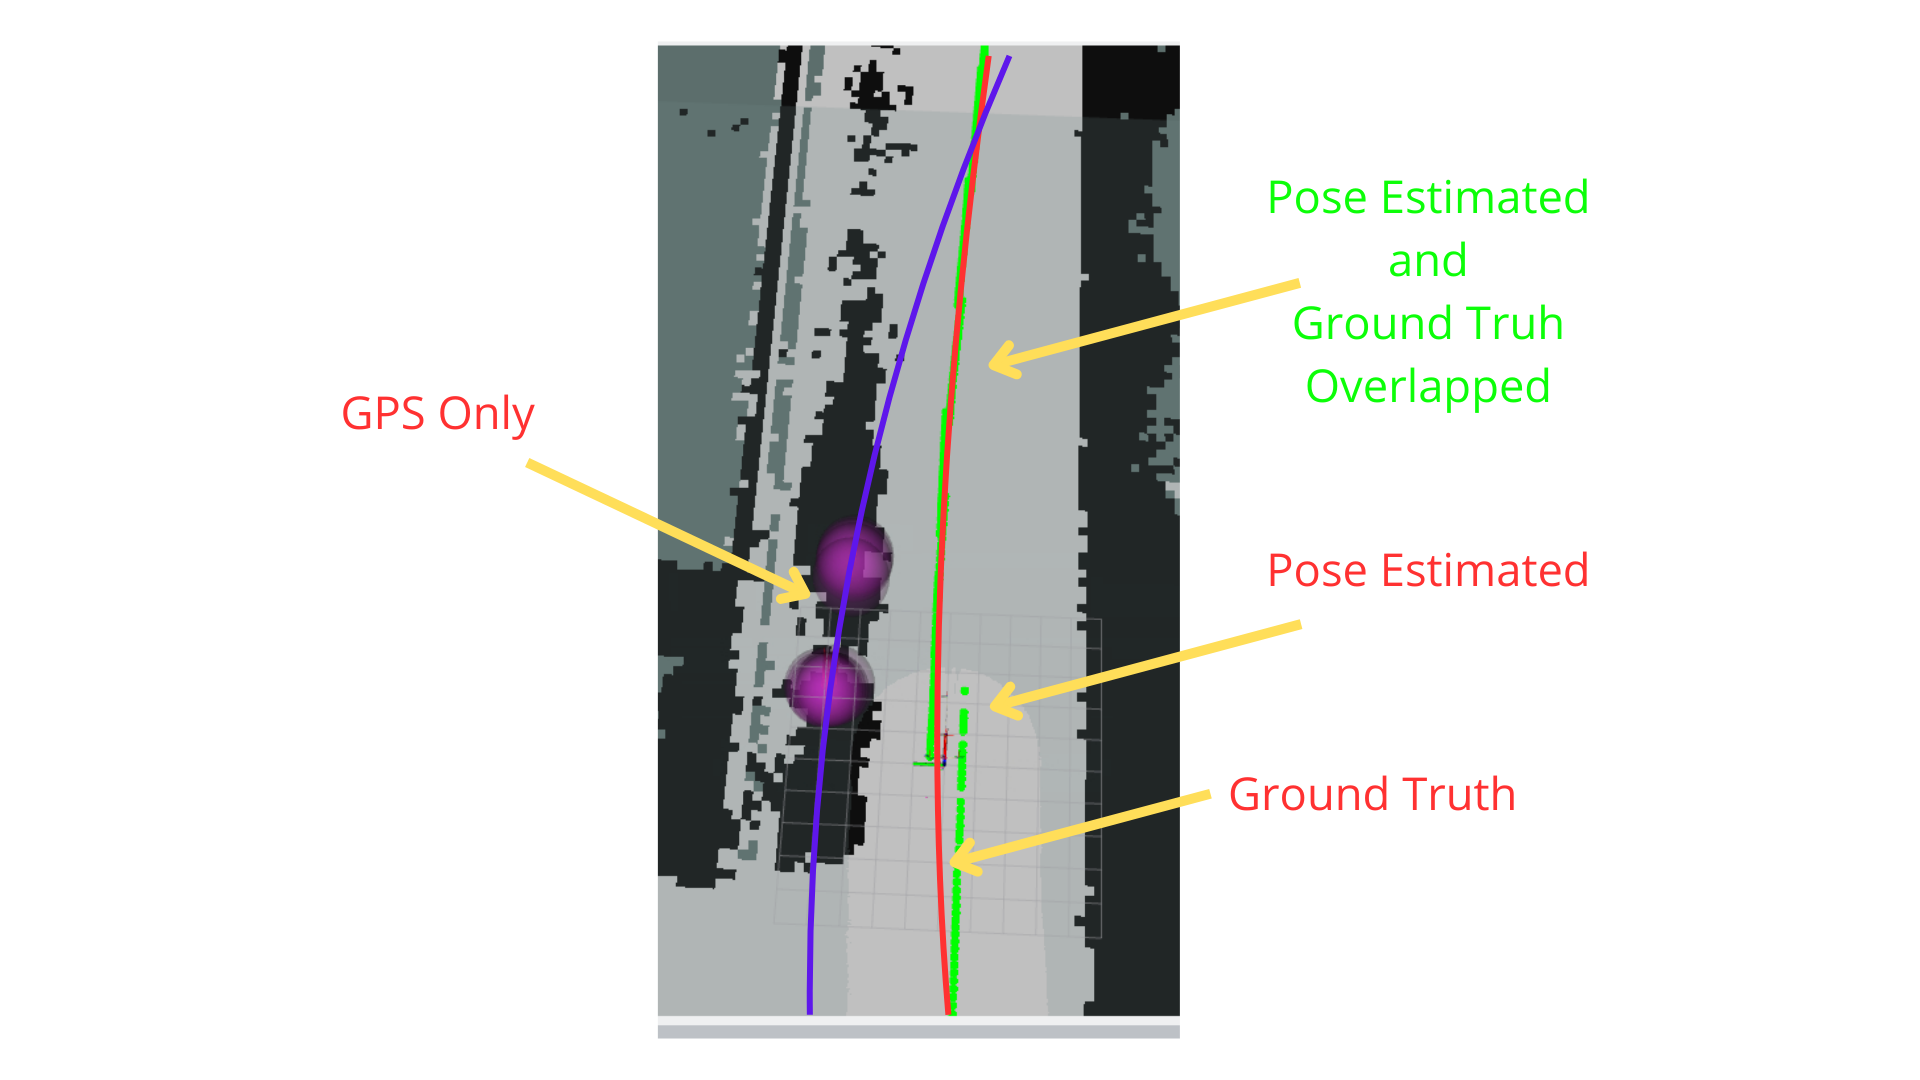
\includegraphics[width=\linewidth]{../konten/acc_asd.png}
        \caption{Accuracy Test of GPS Only vs Graph Based SLAM}
        \label{fig:acc_test}
    \end{figure} 

    Figure \ref{fig:acc_test} shows the accuracy test result of GPS only vs Graph Based SLAM. The purple line shows the GPS only pose estimation, while the green line shows the Graph Based SLAM pose estimation. The red line is the ground truth path that we used to compare the accuracy of both GPS only and Graph Based SLAM. From the figure \ref{fig:acc_test}, we can see that the GPS only has not converged to the ground truth path, while the Graph Based SLAM has converged to the ground truth path. 
    \par    
    From the figure \ref{fig:acc_test}, we can see that the GPS only pose estimation is far better from the ground truth path compared to the Graph Based SLAM pose estimation. In other hand, There is a single jitter that happen on the Graph Based SLAM pose estimation usually because of the sensor synchronization problem for each sensor and the conversion from wheel odometry to the base link car frame. 
}

\newcommand{\PoseEstimationPrecision}{
    \label{sec:pose_est_prec}
    \begin{table}[H]
        \centering
        \caption{Precision Test of GPS Only vs Graph Based SLAM}
        \label{tab:prec_test}
        \begin{tabular}{|c|c|c|c|}
            \hline
            \textbf{GPS x} & \textbf{GPS y} & \textbf{SLAM x} & \textbf{SLAM y} \\ \hline
            0.2 & 0.2 & 0.00 & 0.00 \\ \hline
            0.4 & 0.2 & 0.10 & 0.00 \\ \hline
            0.2 & 0.1 & 0.00 & 0.00 \\ \hline
            0.4 & 0.7 & 0.01 & 0.00 \\ \hline
            1.9 & 1.2 & 0.00 & 0.00 \\ \hline
            1.2 & 0.8 & 0.02 & 0.00 \\ \hline
            1.2 & 0.6 & 0.00 & 0.05 \\ \hline
        \end{tabular}
    \end{table}

    Table \ref{tab:prec_test} shows the precision test result of GPS only vs Graph Based SLAM. The precision test is done by stationary the vehicle in one position and record the pose estimation from GPS only and Graph Based SLAM for 7 times. From the table \ref{tab:prec_test}, we can see that the GPS only has a precision error up to 2.24 meters, while the Graph Based SLAM has a precision error up to 0.10 meters. The standard deviation also can be calculated and have a result 0.69 in GPS only estimation and 0.03 for the graph based slam. This result shows that the Graph Based SLAM has a much better precision than GPS only for navigation system. That can happen because we used the wheel odometry as the main prior for the pose estimation in Graph Based SLAM, so if the vehicle is stationary, the odometry will not change and the pose estimation will be more precise.

    \par   
    The little the standard deviation value, the more stable the system is. So, from the standard deviation result that we have calculated before, we can conclude that the Graph Based SLAM system is more stable than GPS only system for navigation system.
}

\newcommand{\PreviousNavigationSystemvsProposedNavigationSystem}{
    Based on figure \ref{fig:full_system} and figure \ref{fig:full_system_slam} that represent the full navigation system of the previous Icar navigation and the proposed Icar navigation system. The main difference between the previous icar navigation system and the proposed icar navigation system is the dependency to calculate the action of the car. The previous Icar navigation system only uses GPS and odometry to calculate action for velocity and steering, while the proposed Icar navigation system uses complicated sensors and pre-calculated motion for calculating the action for velocity and steering. section \ref{sec:traj_gen} and \ref{sec:safety_system} will discuss about the detail comparison between the previous Icar navigation system and the proposed Icar navigation system.
}

\newcommand{\TrajectoryGeneration}{
    \label{sec:traj_gen}
    The first main part of the autonomous car is the trajectory generation. Based on generated trajectory, the car will calculate the action for velocity and steering. Figure \ref{fig:traj_prev_new} shows the comparison between the previous trajectory generation system and the proposed trajectory generation system that drive on the straight road.

    \begin{figure}[H] 
        \centering
        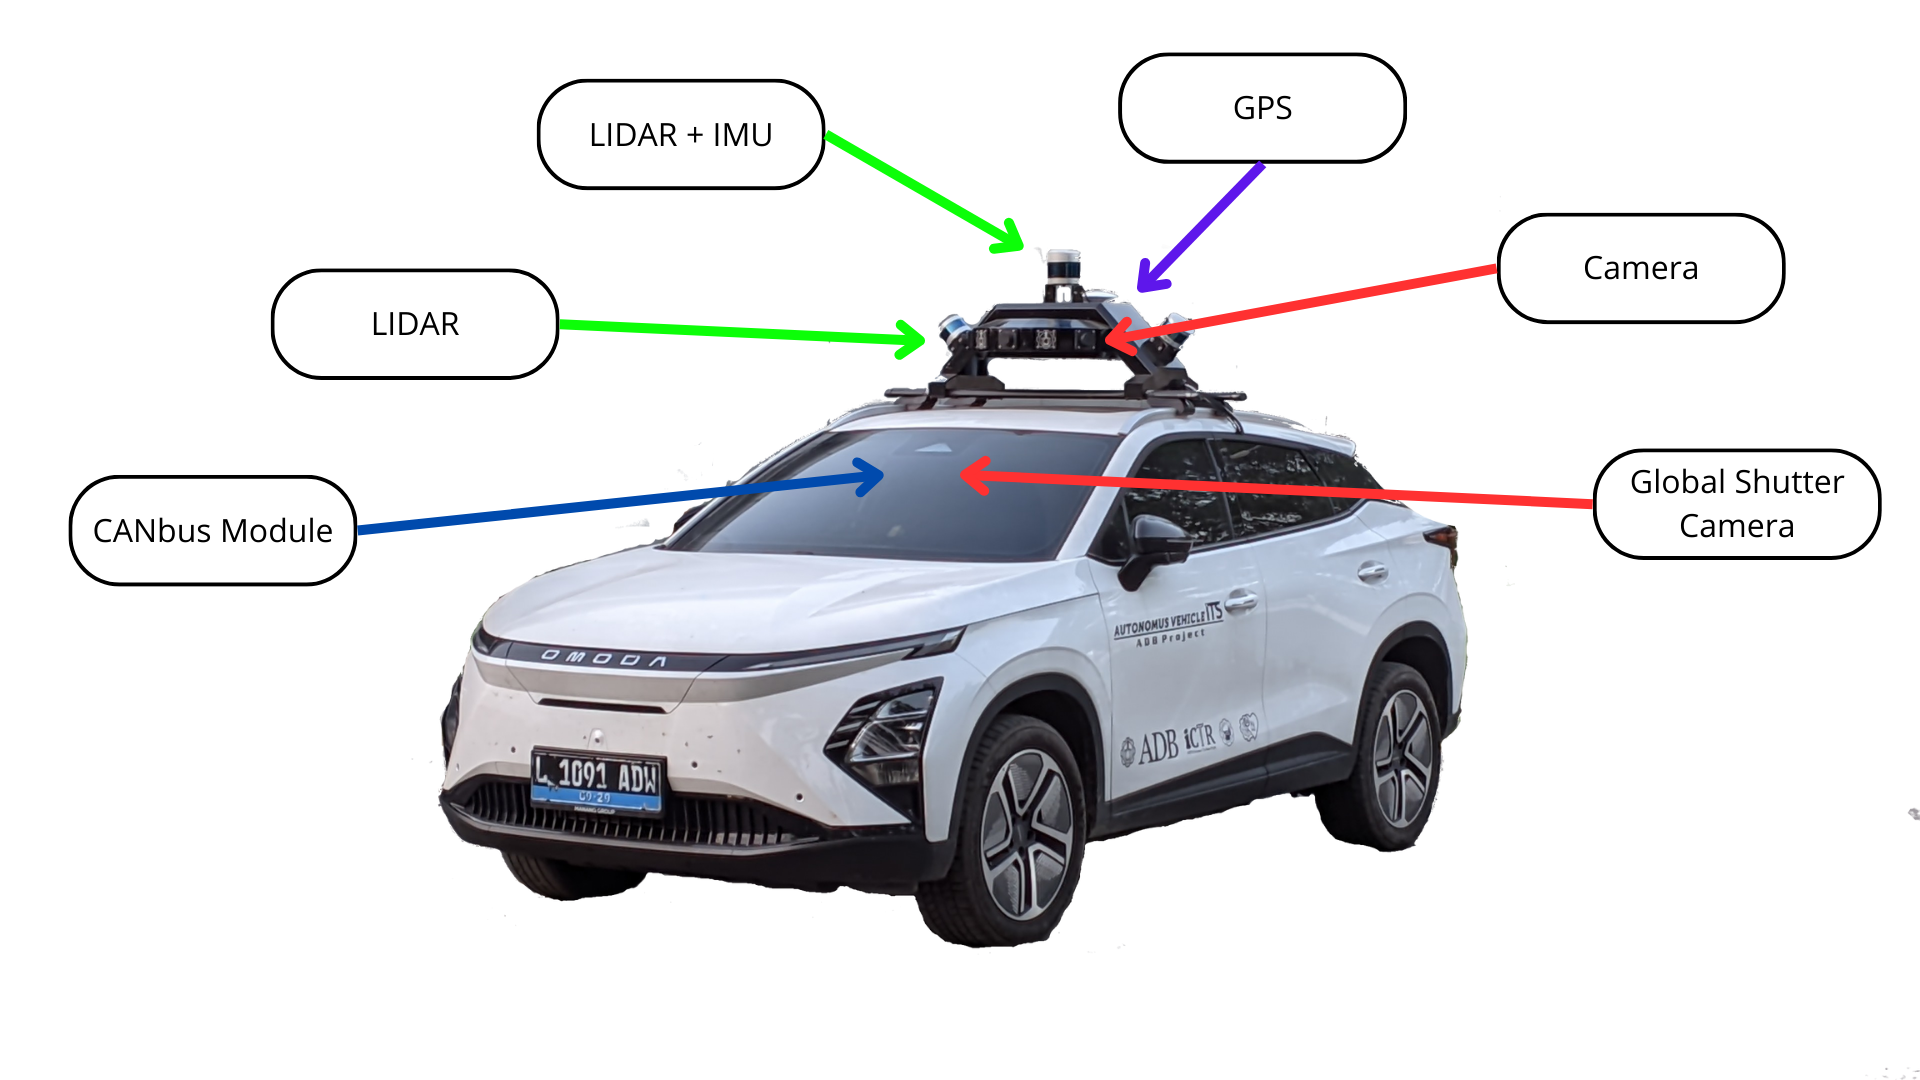
\includegraphics[width=\linewidth]{../konten/local_traj.png}
        \caption{Result of Local Trajectory Generation: Previous vs Proposed}
        \label{fig:traj_prev_new}
    \end{figure} 

    In the figure \ref{fig:traj_prev_new}, the sub image (a) is the previous trajectory generation system and the sub image (b) is the proposed trajectory generation system. From the figure \ref{fig:traj_prev_new}, we can see that the previous trajectory halo halo bandung
}

\newcommand{\SafetySystemResult}{
    \label{sec:safety_system}
    asd asd asd asd asd asd asd asd    
    lorem ipsum dolor sit amet, consectetur adipiscing elit, sed do eiusmod tempor incididunt ut labore et dolore magna aliqua. Ut enim ad minim veniam, quis nostrud exercitation ullamco laboris nisi ut aliquip ex ea commodo consequat. Duis aute irure dolor in reprehenderit in voluptate velit esse cillum dolore eu fugiat nulla pariatur. Excepteur sint occaecat cupidatat non proident, sunt in culpa qui officia deserunt mollit anim id est laborum.
}

\newcommand{\TheImportantofPrediction}{
    asd asd asd asd asd asd asd asd    
    lorem ipsum dolor sit amet, consectetur adipiscing elit, sed do eiusmod tempor incididunt ut labore et dolore magna aliqua. Ut enim ad minim veniam, quis nostrud exercitation ullamco laboris nisi ut aliquip ex ea commodo consequat. Duis aute irure dolor in reprehenderit in voluptate velit esse cillum dolore eu fugiat nulla pariatur. Excepteur sint occaecat cupidatat non proident, sunt in culpa qui officia deserunt mollit anim id est laborum.
}

\newcommand{\AblationStudyonNavigationSystem}{
    Based on the list of tests in \ref{sec:safety_tests}, we have done several ablation studies on the navigation system to find the robustness of the proposed navigation system. 
    \par    
    When the weather become cloudy and low visibility, the road detection still work well because we have added the dataset with cloudy and low visibility condition during the training process. Figure \ref{fig:road_cloudy} shows the result of road detection in cloudy and low visibility condition.
    \begin{figure}[H] 
        \centering
        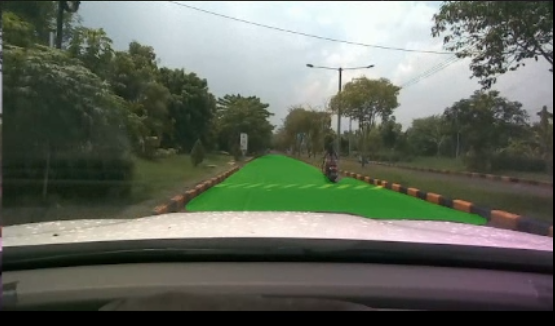
\includegraphics[width=\linewidth]{../konten/seg_gelap.png}
        \caption{Result of Road Detection in Cloudy and Low Visibility Condition}
        \label{fig:road_cloudy}
    \end{figure} 
    Figure \ref{fig:road_cloudy} shows that the road detection still work well in cloudy and low visibility condition. The green area is the detected road area. 
    \par    
    
    \begin{figure}[H] 
        \centering
        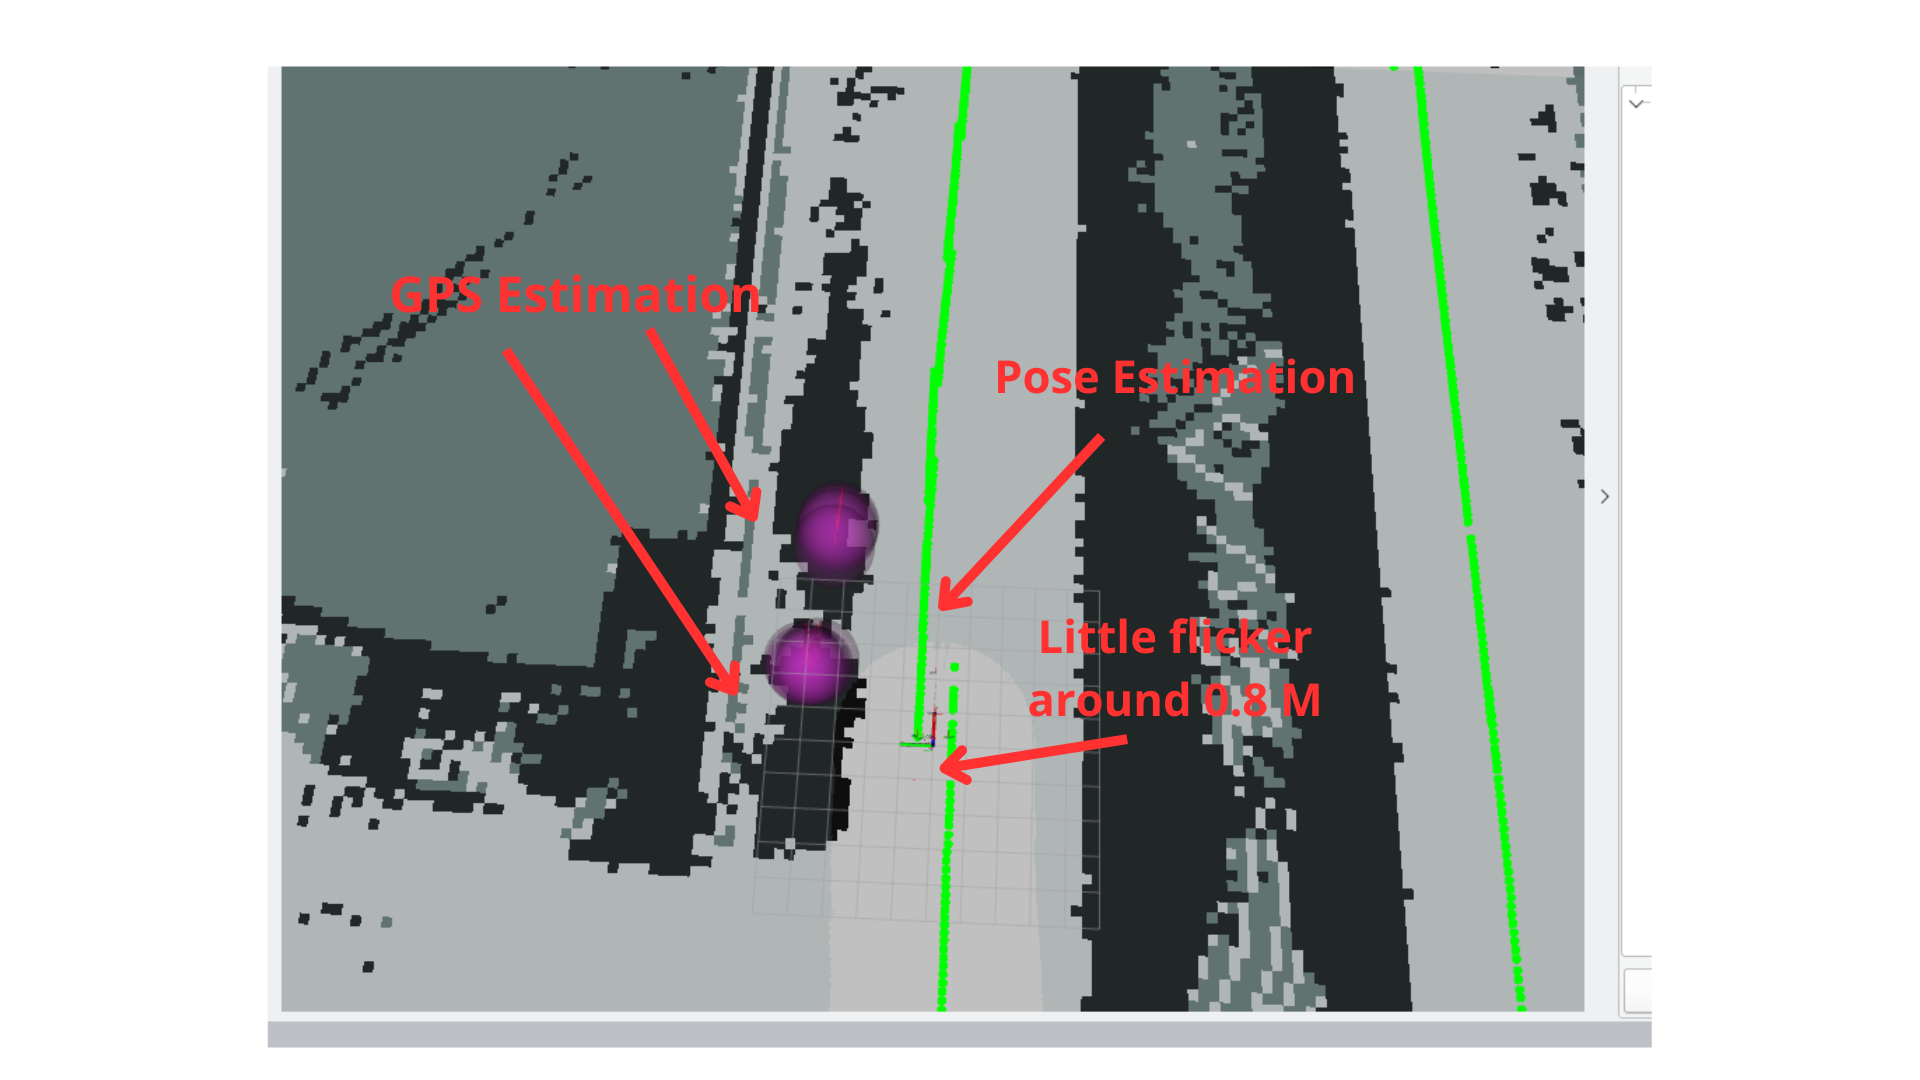
\includegraphics[width=\linewidth]{../konten/multipath.png}
        \caption{Result of Pose Estimation in Multipath GPS Condition}
        \label{fig:pose_multipath}
    \end{figure} 
    Figure \ref{fig:pose_multipath} shows the result of pose estimation in multipath GPS condition. The multipath GPS condition represented by the sphere purple area. The pose estimation represented by the green line. From the figure \ref{fig:pose_multipath}, we can see that the pose estimation still work well in multipath GPS condition because even through there still a little jitter on the pose estimation around 0.5 meter. 

    \par  
    When there is a jitter pose estimation happen like in figure \ref{fig:pose_multipath}, the navigation system still navigate well because have applied an $\alpha$-$\beta$-$\gamma$ filter to smooth the trajectory.
}